\documentclass[../Notas.tex]{subfiles}
\graphicspath{{\subfix{../images/}}}

\begin{document}

%\section{Tópico 5}

\section{Variáveis aleatórias contínuas}
Vimos situações em que as v.a.'s representavam o número de ``objetos'' ou ``coisas''. Entretanto, há muitas situações (tanto teóricas quanto práticas) em que a v.a. natural a se considerar é ``contínua'' num certo sentido, e.g. o tempo que decorre até a recuperação completa de um paciente com determinada doença.

\begin{definition}[V.a. contínua]
Uma v.a. $X$ em $(\Omega, \mathcal{A}, P)$ é dita \textbf{contínua} se $P(X=x) = 0, \forall x\in\mathbb{R}$.
\end{definition}

Recordando das propriedades da f.d. de uma v.a., temos o seguinte fato.

\begin{proposition}
$X$ é v.a. contínua se, e só se, $F_X$ é contínua.
\end{proposition}

\begin{proof}
Dado $x\in\mathbb{R}$,
\begin{align*}
    0 = P(X=x) = F_X(x) - F_X(x^-) \iff F_X(x^+) = F_X(x) = F_X(x^-).
\end{align*}
\end{proof}

No caso de v.a.'s contínuas, podemos trocar os sinais $<$ e $\leq$ à vontade nos cálculos de probabilidades.

\begin{example}
Considere o experimento de escolher um ponto ao acaso no círculo de centro na origem e raio $R>0$ (jogar um dardo). Vimos que, nesse caso, um espaço de probabilidade adequado é $(\Omega, \mathcal{A}, P)$ com
\begin{align*}
    \Omega = \{ (x,y)\in\mathbb{R}^2 : x^2+y^2\leq R^2 \}, \mathcal{A} = \mathcal{B}^2(\Omega)
\end{align*}
e $P:\mathcal{A}\to\mathbb{R}$ tal que
\begin{align*}
    P(A) = \iint_A \frac{1}{\pi R^2}dxdy, \forall A\in\mathcal{A}.
\end{align*}
Podemos definir a v.a. $X:\Omega\to\mathbb{R}$ por $X(\omega) = X((x,y)) = \sqrt{x^2+y^2}$. Note que, dado $z\in\mathbb{R}$, temos $\{X = z\} = \emptyset$ se $z < 0$ ou $z>R$ e $\{ X=z \} = \{ (x,y)\in\Omega : x^2+y^2 = z^2 \}$ se $0\leq z \leq R$. Logo, $P(X=z) = 0, \forall z\in\mathbb{R}$, ou seja, $X$ é v.a. contínua. Por outro lado, $\{X\leq z\} = \emptyset$ se $z<0$, $\{X\leq z\} = \{ (x,y)\in\Omega : x^2+y^2 \leq z^2 \}$ se $0\leq z < R$ e $\{X\leq z\} = \Omega$ se $z\geq R$. Logo,
\begin{align*}
    F_X(z) = \begin{cases}
    0, z < 0 \\
    z^2/R^2, 0\leq z < R \\
    1, z\geq R
    \end{cases}.
\end{align*}
Em particular, se $0\leq a < b\leq R$, então
\begin{align*}
    P(a < X < b) = F_X(b) - F_X(a) = \frac{b^2 - a^2}{R^2} > 0.
\end{align*}
\begin{figure}[H]
    \centering
    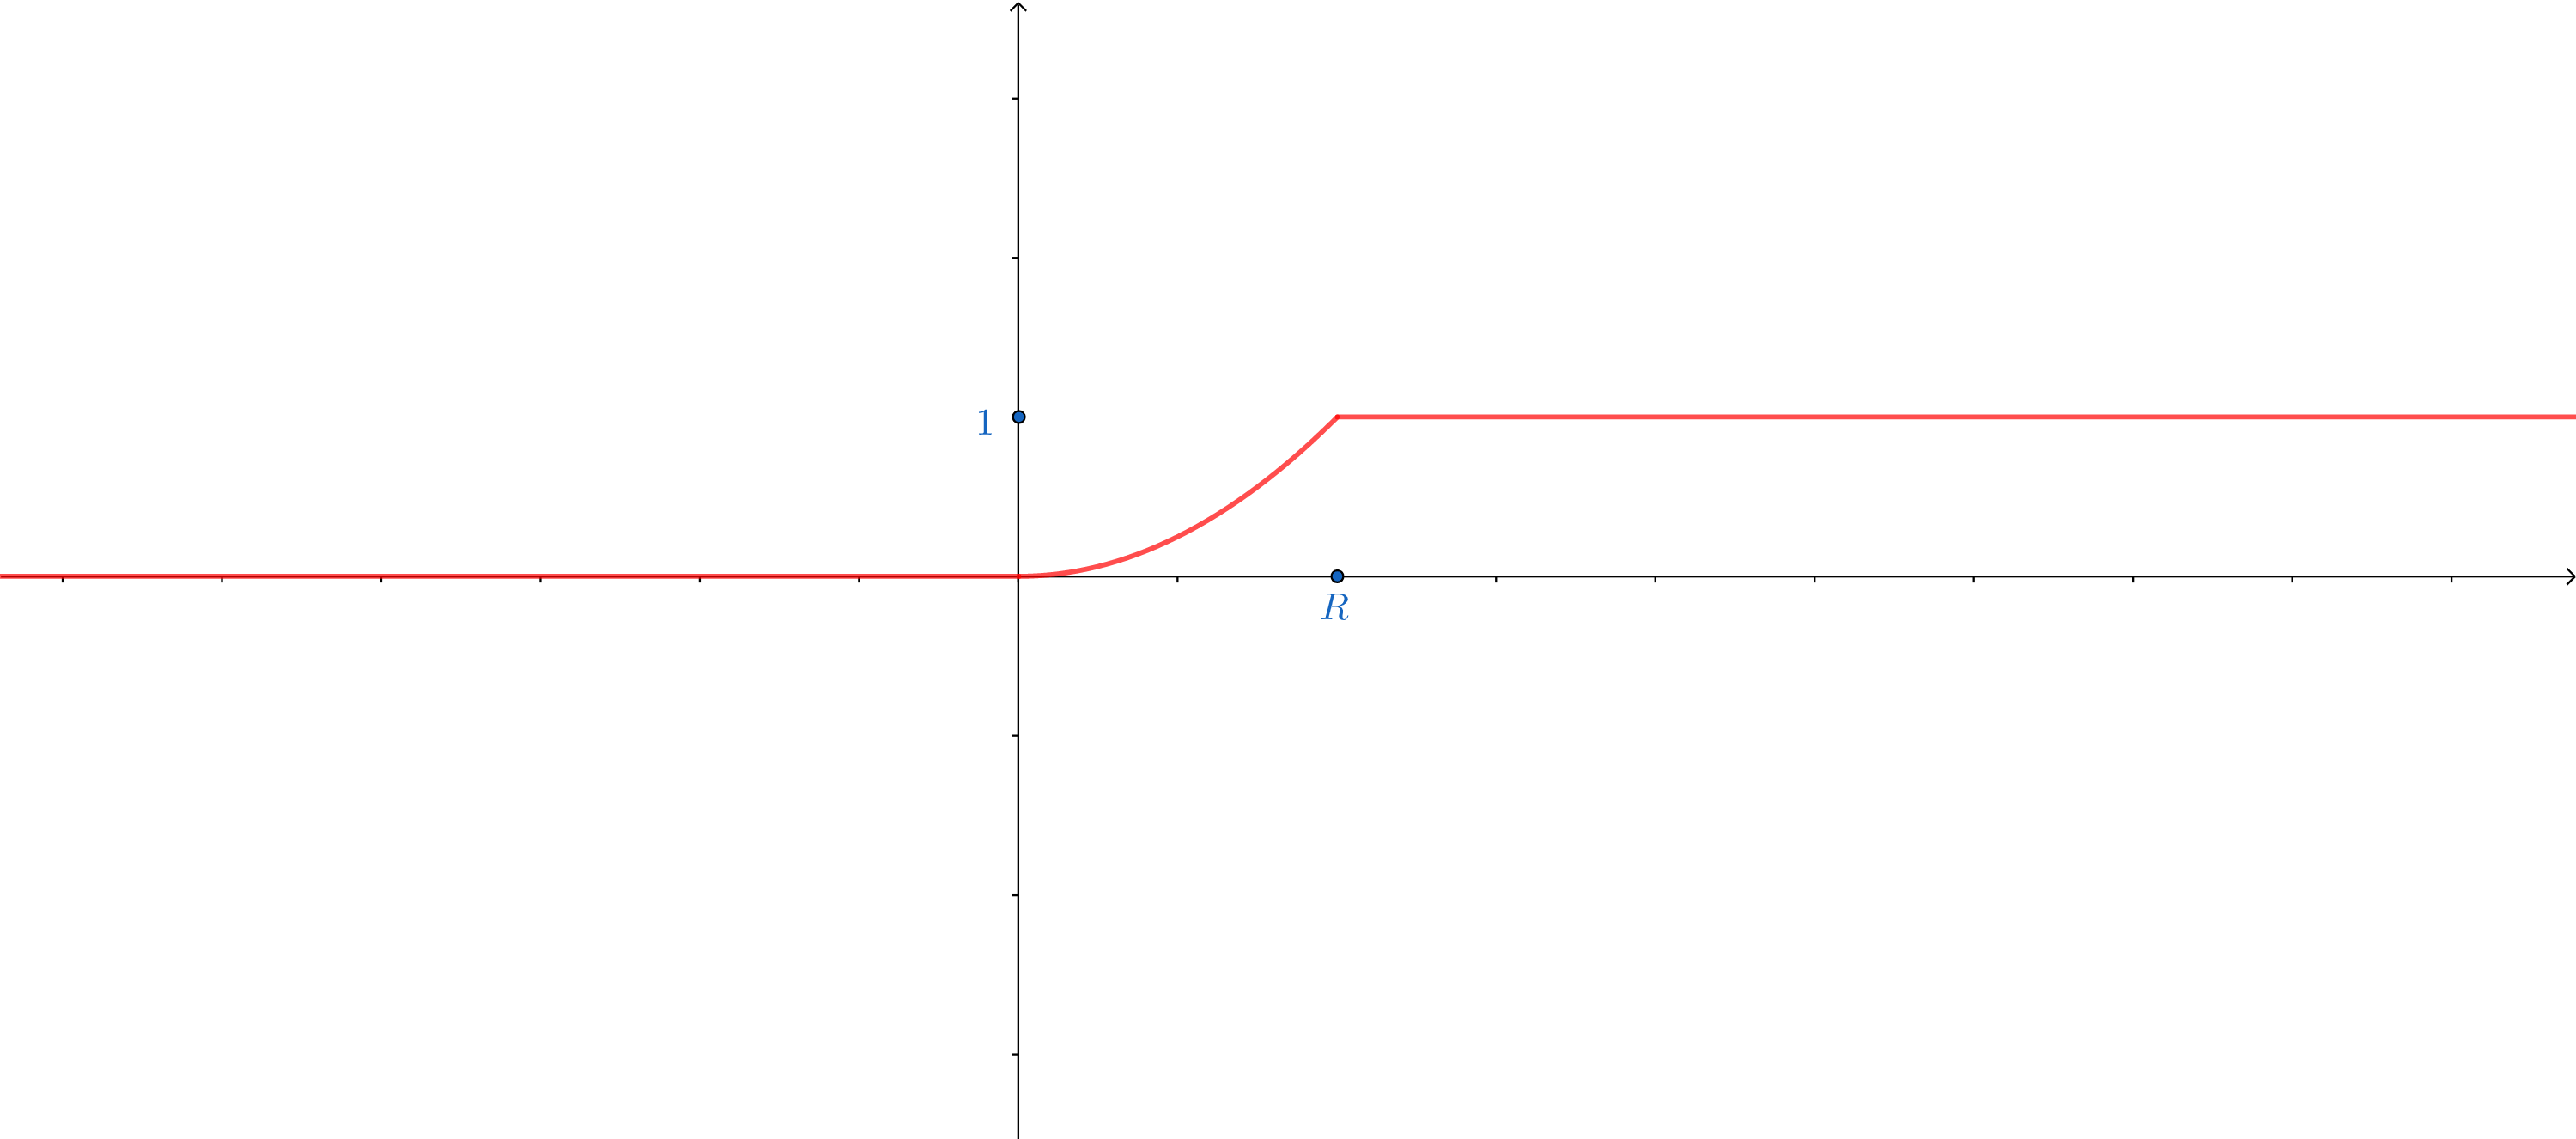
\includegraphics[width=\textwidth]{Imagens/p104.png}
    \caption{Gráfico da f.d. anterior}
%    \label{fig:my_label}
\end{figure}
\end{example}

\begin{definition}[Função de densidade]
Uma função $f:\mathbb{R}\to\mathbb{R}$ tal que
\begin{enumerate}[(i)]
    \item $f(x)\geq 0, \forall x\in\mathbb{R}$ 
    \item $\displaystyle{ \int_{\mathbb{R}} f(x)dx  = 1}$
\end{enumerate}
é dita \textbf{função de densidade de probabilidade} ou apenas \textbf{densidade}.
\end{definition}

\begin{definition}[Função de distribuição]
Uma função $F:\mathbb{R}\to\mathbb{R}$ tal que
\begin{align*}
    F(x) = \int_{-\infty}^x f(t) dt, \forall x\in\mathbb{R}
\end{align*}
para alguma densidade $f$ é dita \textbf{função de distribuição (absolutamente) contínua}. Dizemos ainda que $f$ é a densidade de $F$.
\end{definition}

\begin{remark}
É possível, mas complicado, construir exemplos de funções $F$ que sejam contínuas mas não tenham densidade. As que têm densidade são chamadas de \textbf{absolutamente} contínuas. Aqui não faremos distinção, pois os casos não absolutamente contínuos são raros; sempre que nos referirmos a uma f.d., estará implícito que ela é absolutamente contínua.

Outro ponto importante é que dada $F$, a densidade $f$ não é única, já que $F$ pode não ser derivável. Contudo, os pontos onde $F$ não é derivável (ou onde $f$ não é contínua) formam um conjunto enumerável, de maneira que a integral não se altera. Em geral é comum tomar $f$ como
\begin{align*}
    f(x) = \begin{cases}
    F'(x), \forall x\in\mathbb{R} : \exists F'(x) \\
    0, \text{ c.c.}
    \end{cases}
\end{align*}
\end{remark}

\begin{definition}
Uma v.a. $X$ definida em $(\Omega, \mathcal{A}, P)$ é \textbf{(absolutamente) contínua} se sua f.d. $F_X$ é \textbf{(absolutamente) contínua}, i.e., se $F_X(x) = \displaystyle{ \int_{-\infty}^x f(t)dt, \forall x\in\mathbb{R} }$ para alguma função de densidade $f:=f_X$, chamada \textbf{densidade} de $X$.
\end{definition}

\begin{remark}
Como no caso discreto, podemos nos referir tanto a $F_X$ quanto a $f_X$ quando dizemos ``distribuição'', devido à relação biunívoca entre ambas as funções. Além disso, se $X$ é v.a. contínua com densidade $f_X$, então dados $a,b\in\mathbb{R}$ quaisquer com $a\leq b$, temos
\begin{align*}
    P(a < X < b) = F_X(b) - F_X(a) = \int_a^b f_X(x) dx,
\end{align*}
ou seja, $P(a < X < b)$ é a área da região $A$.
\begin{figure}[H]
    \centering
    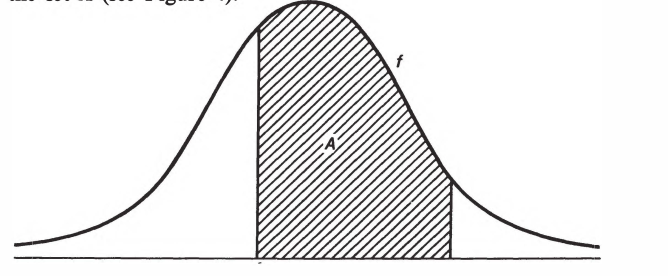
\includegraphics[width=\textwidth]{Imagens/p105.png}
    \caption{Gráfico obtido de \cite{Hoel}.}
%    \label{fig:my_label}
\end{figure}
\end{remark}

\begin{example}
No exemplo do dardo acima, vimos que
\begin{align*}
    F_X(x) = \begin{cases}
    0, x < 0 \\
    x^2/R^2, 0\leq x < R \\
    1, x\geq R
    \end{cases}.
\end{align*}
Logo, a densidade $f$ de $X$ é
\begin{align*}
    f_X(x) = \begin{cases}
    0, x < 0 \\
    2x/R^2, 0\leq x < R \\
    0, x\geq R
    \end{cases}.
\end{align*}
Note que não existe $F'_X(R)$, pois $F_{X_-}'(R) = 2/R \neq 0 = F'_{X_+}(R)$, ou seja, $f$ não é contínua em $R$. Assim, sem perda de generalidade, tomamos $f(R) = 0$, de modo que
\begin{align*}
    f_X(x) = \begin{cases}
    2x/R^2, 0\leq x < R \\
    0, \text{ c.c.}
    \end{cases}
\end{align*}
e ainda vale $\displaystyle{ F_X(x) = \int_{-\infty}^x f_X(t) dt, \forall x\in\mathbb{R}. }$
\end{example}

\begin{remark}
É importante notar que há v.a.'s que não são nem contínuas nem discretas, chamadas \textbf{mistas}. Por exemplo, a v.a. $X$ com f.d. $F_X$ dada pelo gráfico abaixo não é contínua, pois $F_X$ é descontínua em $a$; entretanto, $X$ tampouco é discreta, pois $F_X$ não é do tipo escada.
\begin{figure}[H]
    \centering
    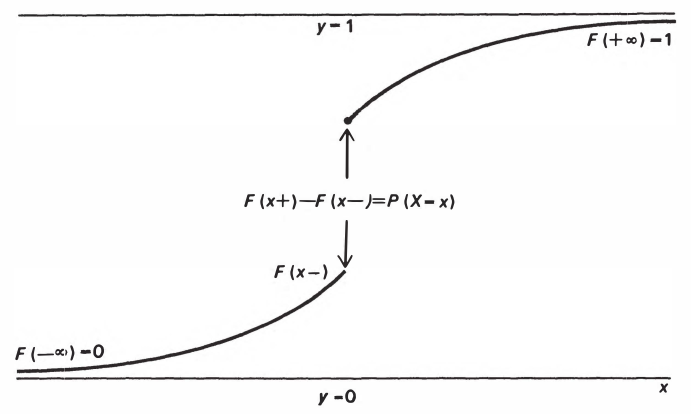
\includegraphics[width=\textwidth]{Imagens/p106-1.png}
    \caption{Gráfico obtido de \cite{Hoel}.}
%    \label{fig:my_label}
\end{figure}
\end{remark}

\begin{definition}
Seja $X$ uma v.a.; dizemos que
\begin{enumerate}[(i)]
    \item $X$ é simétrica em torno de 0 se $P(X\geq x) = P(X\leq -x), \forall x\in\mathbb{R}$, i.e., $X$ e $-X$ têm a mesma distribuição;
    \item $X$ é simétrica em torno de $\mu$ se existe $\mu\in\mathbb{R}$ tal que $P(X\geq \mu + x) = P(X\leq \mu - x), \forall x\in\mathbb{R}$.
\end{enumerate}
\end{definition}

\begin{theorem}
Seja $X$ v.a. contínua com densidade $f$. Então $X$ é simétrica em torno de 0 se, e só se, $f$ é par; nesse caso, $f$ é \textbf{densidade simétrica}. De modo geral, $X$ é simétrica em torno de $\mu\in\mathbb{R}$ se, e só se, $f(\mu + x) = f(\mu - x)$. Nesse caso, $f$ é \textbf{densidade simétrica em torno de} $\mu$.
\end{theorem}

\begin{proof}
Provamos em torno de 0. Se $f$ é par, então
\begin{align*}
    P(X\geq x) = \int_x^{\infty} f(t)dt = \int_{-\infty}^{-x} f(-y)dy = \int_{-\infty}^{-x} f(y)dy = P(X\leq -x),
\end{align*}
logo $X$ é simétrica. Reciprocamente, se $P(X\geq x) = P(X\geq -x)$, defina
\begin{align*}
    g(x) = \frac{f(x) + f(-x)}{2}.
\end{align*}
Note que $g$ é simétrica, logo
\begin{align*}
    \int_{-\infty}^x g(y) dy &= \frac{1}{2}\int_{-\infty}^x f(y) dy + \frac{1}{2}\int_{-\infty}^x f(-y) dy \\
    &= \frac{1}{2}\int_{-\infty}^x f(y) dy + \frac{1}{2}\int_{-x}^{\infty} f(y) dy \\
    &= \frac{1}{2}P(X\leq x) + \frac{1}{2}P(-X\geq -x) \\
    &= P(X\leq x),
\end{align*}
ou seja, $X$ tem densidade $g$ simétrica. A demonstração do caso geral é análoga, substituindo $x$ por $x+\mu$.
\end{proof}

\begin{remark}
É possível mostrar que o resultado acima vale também para v.a.'s discretas; além disso, note que se $X$ é simétrica em torno da origem então $F(0) = 1/2$ e, se $X$ é simétrica em torno de $\mu$, então $F(\mu) = 1/2$. De maneira geral, se $X$ é simétrica em torno da origem então
\begin{align*}
    F(-x) = \int_{-\infty}^{-x}f(y) dy = \int_x^{\infty} f(-y)dy = \int_x^{\infty} f(y) dy = \int_{-\infty}^{\infty} f(y) dy - \int_{-\infty}^x f(y) dy,
\end{align*}
ou seja, $F(-x) = 1 - F_X(x), \forall x\in\mathbb{R}$.
\end{remark}

\subsection{Exemplos clássicos de distribuições contínuas}
\begin{example}[Uniforme contínua, $X\sim U(a,b)$]
Dizemos que $X$ é uma v.a. contínua com distribuição uniforme no intervalo $(a,b)$ se tem densidade dada por
\begin{align*}
    f(x) = \begin{cases}
    \frac{1}{b-a}, a < x < b \\
    0, \text{ c.c.}
    \end{cases}.
\end{align*}
Note que $f(x)\geq 0, \forall x\in\mathbb{R}$ e $\displaystyle{ \int_{\mathbb{R}} f(x) dx = 1 }$. A f.d. $F$ associada a $f$ é calculada como segue:
\begin{align*}
    F(x) &= \int_{-\infty}^x f(t) dt = 0, x < a \\
    F(x) &= \int_{-\infty}^x f(t) dt = \int_a^x \frac{1}{b-a} dt = \frac{x-a}{b-a}, a\leq x < b \\
    F(x) &= \int_{-\infty}^x f(t) dt = \int_a^b \frac{1}{b-a} dt = 1, x \geq b, 
\end{align*}
ou seja,
\begin{align*}
    F(x) = \begin{cases}
    0, x<a \\
    \frac{x-a}{b-a}, a\leq x < b \\
    1, x\geq b
    \end{cases}.
\end{align*}
Note também que $f(x) = F'(x), \forall x\in\mathbb{R}\setminus\{a,b\}$.
\end{example}

\begin{example}[Exponencial, $X\sim\text{Exp}(\lambda)$]
Dizemos que $X$ é uma v.a. contínua com distribuição exponencial de parâmetro $\lambda > 0$ se tem densidade dada por
\begin{align*}
    f(x) = \begin{cases}
    \lambda e^{-\lambda x}, x > 0 \\
    0, x \leq 0
    \end{cases}
\end{align*}
ou, equivalentemente, f.d. dada por
\begin{align*}
    F(x) = \begin{cases}
    1 - e^{-\lambda x}, x > 0 \\
    0, x\leq 0
    \end{cases}.
\end{align*}
Note que, de fato, $f(x) \geq 0, \forall x\in\mathbb{R}$ e que
\begin{align*}
    \int_{\mathbb{R}} f(t) dt = \int_0^{+\infty} \lambda e^{-\lambda t} dt = 1.
\end{align*}
Ademais, $f(x) = F'(x), \forall x\in\mathbb{R}\setminus\{0\}$.
\end{example}

\begin{remark}
A distribuição exponencial é utilizada muitas vezes quando a v.a. em questão é um tempo de espera, e.g. o tempo até que um componente eletrônico apresente falhas. Além disso, se $X\sim\text{Exp}(\lambda)$, então $X$ tem perda de memória, i.e., $P(X > a+b) = P(X>a)P(X>b), a,b\geq 0$ ou, equivalentemente, $P(X>a+b| X>a) = P(X>b), a,b\geq 0$.
\begin{proof}
De fato, se $X\sim\text{Exp}(\lambda)$, então
\begin{align*}
    P(X>a+b|X>a) &= \frac{P(X>a+b, X>a)}{P(X>a)} \\
    &= \frac{P(X>a+b)}{P(X>a)} \\
    &= \frac{ e^{-\lambda (a+b)} }{ e^{-\lambda a} } \\
    &= e^{-\lambda b} \\
    &= P(X>b), \forall a,b\geq 0.
\end{align*}
\end{proof}
Na verdade, a v.a. exponencial é a única v.a. contínua não negativa com perda de memória.
\end{remark}

\begin{theorem}
$X$ é v.a. contínua com perda de memória se, e só se, $X\sim\text{Exp}(\lambda)$ para algum $\lambda > 0$ ou $P(X>0) = 0$.
\end{theorem}

\begin{proof}
($\Leftarrow$) Já vimos o caso que $X$ tem distribuição exponencial; se $P(X>0) = 0$, então $P(X > a+b) = 0 = P(X>a)P(X>b), \forall a,b\geq 0$.

($\Rightarrow$) Se $X$ tem perda de memória e $P(X > 0) \neq 0$, então tomando $a = 0 = b$ segue que
\begin{align*}
    P(X>0) = [P(X>0)]^2 \implies P(X > 0) = 1, 
\end{align*}
ou seja, $X$ é v.a. positiva. Seja $F$ a f.d. de $X$ e defina $G(x) = 1 - F(x)$. Temos $G$ não crescente, contínua à direita, $G(0) = 1, G(+\infty) = 0$ e $G(a+b) = G(a)G(b), \forall a,b>0$. Daí, se $c\in\mathbb{R}^*_+$ e $m,n\in\mathbb{R}$, temos
\begin{align*}
    G(c) = G(c - c/m)G(c/m) = G(c - 2c/m)[G(c/m)]^2 = \cdots = G(0)[G(c/m)]^m = [G(c/m)]^m,
\end{align*}
donde segue que
\begin{align*}
    G(nc) = [G(c)]^n.
\end{align*}
Além disso, temos $0 < G(1) < 1$. De fato, se $G(1) = 1$ então teríamos
\begin{align*}
    G(n) = [G(1)]^n \implies G(+\infty) = 1,
\end{align*}
absurdo. Se $G(1) = 0$, então teríamos
\begin{align*}
    G(1/m) = 0 \implies G(0) = G(0^+) = \lim_{m\to +\infty} G(1/m) = \lim_{m\to +\infty} [G(1)]^{1/m} = 0,
\end{align*}
absurdo. Logo, como $0 < G(1) < 1$, podemos tomar $G(1) = e^{-\lambda}$, para algum $\lambda > 0$. Tomando $c=1$, segue que $G(1/m) = e^{-\lambda /m}, m\in\mathbb{N}$ e, fazendo $c = 1/m$, temos $G(n/m) = [G(1/m)]^n = e^{-\lambda n/m}, \forall n,m\in\mathbb{N}$. Logo, $G(y) = e^{-\lambda y}, \forall y\in\mathbb{Q}$. Da continuidade à direita, temos
\begin{align*}
    G(x) = \lim_{y\to x^+, y\in\mathbb{Q}} G(y) = e^{-\lambda x}, \forall x\in\mathbb{R}^*_+,
\end{align*}
pois $\mathbb{Q}$ é denso em $\mathbb{R}$. Daí, segue que $F(x) = 1 - e^{-\lambda x}, \forall x>0$, ou seja, $X\sim\text{Exp}(\lambda)$.
\end{proof}

\begin{remark}
Além de tempo de falha, variáveis exponenciais são úteis para estudar o tempo de decaimento de uma partícula radioativa e, também, no estudo de processos de Poisson e cadeias de Markov. Ademais, pensando na variável exponencial como o tempo de falha, a propriedade de perda de memória diz que dado que não houve falha até o tempo $a$, a probabilidade de que não haja falha nas próximas $b$ unidades de tempo é igual à probabilidade incondicional de que não haja falha nas primeiras $b$ unidades de tempo. Isso implica que o desgaste de uma peça de equipamento não aumenta nem diminui a probabilidade de falha em um dado intervalo de tempo.
\end{remark}

\begin{example}[Normal/gaussiana]
Dizemos que $X$ é v.a. com distribuição normal \textbf{padrão}, $X\sim N(0,1)$, se tem densidade dada por
\begin{align*}
    f(x) = \frac{1}{\sqrt{2\pi}}e^{-x^2/2}, x\in\mathbb{R}.
\end{align*}
\begin{proof}
Vamos mostrar que $f$ de fato é densidade. Primeiro, $f(x) > 0, \forall x\in\mathbb{R}$. Ademais, vamos verificar que $\displaystyle{ \int_{\mathbb{R}} f(x) dx = 1 }$. Seja $g(x) = e^{-x^2/2}, x\in\mathbb{R}$. Note que $g$ é par, contínua e não negativa. Além disso, se $x\geq 1$ então $0 < g(x) < e^{-x/2}$ e, então,
\begin{align*}
    \int_{1}^{\infty} e^{-x^2/2} dx \leq \int_{1}^{\infty} e^{-x/2} dx = \lim_{a\to +\infty} \int_{1}^{a} e^{-x/2} dx = \lim_{a\to +\infty} -2e^{-x/2}\Big|_{1}^a = 2e^{-1/2}\in\mathbb{R},
\end{align*}
logo $\displaystyle{ \int_{1}^{\infty} e^{-x^2/2} dx \in\mathbb{R}}$. Como $g$ é par, temos $\displaystyle{ \int_{1}^{\infty} e^{-x^2/2} dx = \int_{-\infty}^{-1} e^{-x^2/2} dx \in\mathbb{R}}$ e, como $g$ é contínua em $\mathbb{R}$, temos também $\displaystyle{ \int_{-1}^{1} e^{-x^2/2} dx \in\mathbb{R}}$. Logo, $\displaystyle{ \int_{-\infty}^{\infty} e^{-x^2/2} dx \in\mathbb{R}}$, digamos $c$. Segue então que
\begin{align*}
    c^2 = \int_{-\infty}^{\infty} e^{-x^2/2} dx\int_{-\infty}^{\infty} e^{-y^2/2} dy = \iint_{\mathbb{R}^2} e^{-\frac{x^2+y^2}{2}} dxdy = \int_{0}^{\infty}\int_{0}^{2\pi} re^{-r^2/2} drd\theta = 2\pi \int_{0}^{\infty} re^{-r^2/2} dr = 2\pi,
\end{align*}
ou seja, $c = \sqrt{2\pi}$, pois $c>0$. Logo, $\displaystyle{ \int_{\mathbb{R}} f(x) dx = \frac{1}{\sqrt{2\pi}} \int_{\mathbb{R}} g(x) dx = 1.}$ Note que $f$ é simétrica em torno de 0 e, além disso, a f.d. $F$ associada a $f$ é dada por
\begin{align*}
    F(x) = \int_{-\infty}^x \frac{1}{\sqrt{2\pi}} e^{-t^2/2} dt, x\in\mathbb{R}.
\end{align*}
Verifica-se que $F$ não tem uma forma fechada, mas podemos aproximar seus valores numericamente. Como mencionado antes, temos $F(0) = 1/2 = 1 - F(0)$ e $F(x) = 1 - F(x), \forall x\in\mathbb{R}$. É comum também denotar $f$ por $\varphi$ e $F$ por $\Phi$ no caso da densidade e da f.d. de uma v.a. normal padrão, respectivamente.
\end{proof}
\begin{remark}
Tabelas de valores para a distribuição normal geralmente fornecem as probabilidades do tipo $P(0 < X < a)$. De fato, basta apenas esta probabilidade, pois $P(X\leq a) = 1/2 + P(0 < X < a), a>0$ e analogamente para os demais casos.
\end{remark}
De maneira geral, dizemos que $X$ é v.a. contínua com distribuição \textbf{normal de parâmetros} $\mu$ \textbf{e} $\sigma^2$, $X\sim N(\mu, \sigma^2)$ (veremos o que esses parâmetros significam mais à frente), se tem densidade dada por
\begin{align*}
    f(x) = \frac{1}{\sqrt{2\pi}\sigma}e^{-\frac{(x-\mu)^2}{2\sigma^2}}, x\in\mathbb{R},
\end{align*}
com $\mu,\sigma\in\mathbb{R}$ e $\sigma>0$. A verificação de que $f$ de fato é densidade é análoga ao que fizemos acima, bastando apenas efetuar a mudança de variável $y = \displaystyle{\frac{x-\mu}{\sigma}}$. Note também que $f$ é simétrica em torno de $\mu$.
\begin{figure}[H]
    \centering
    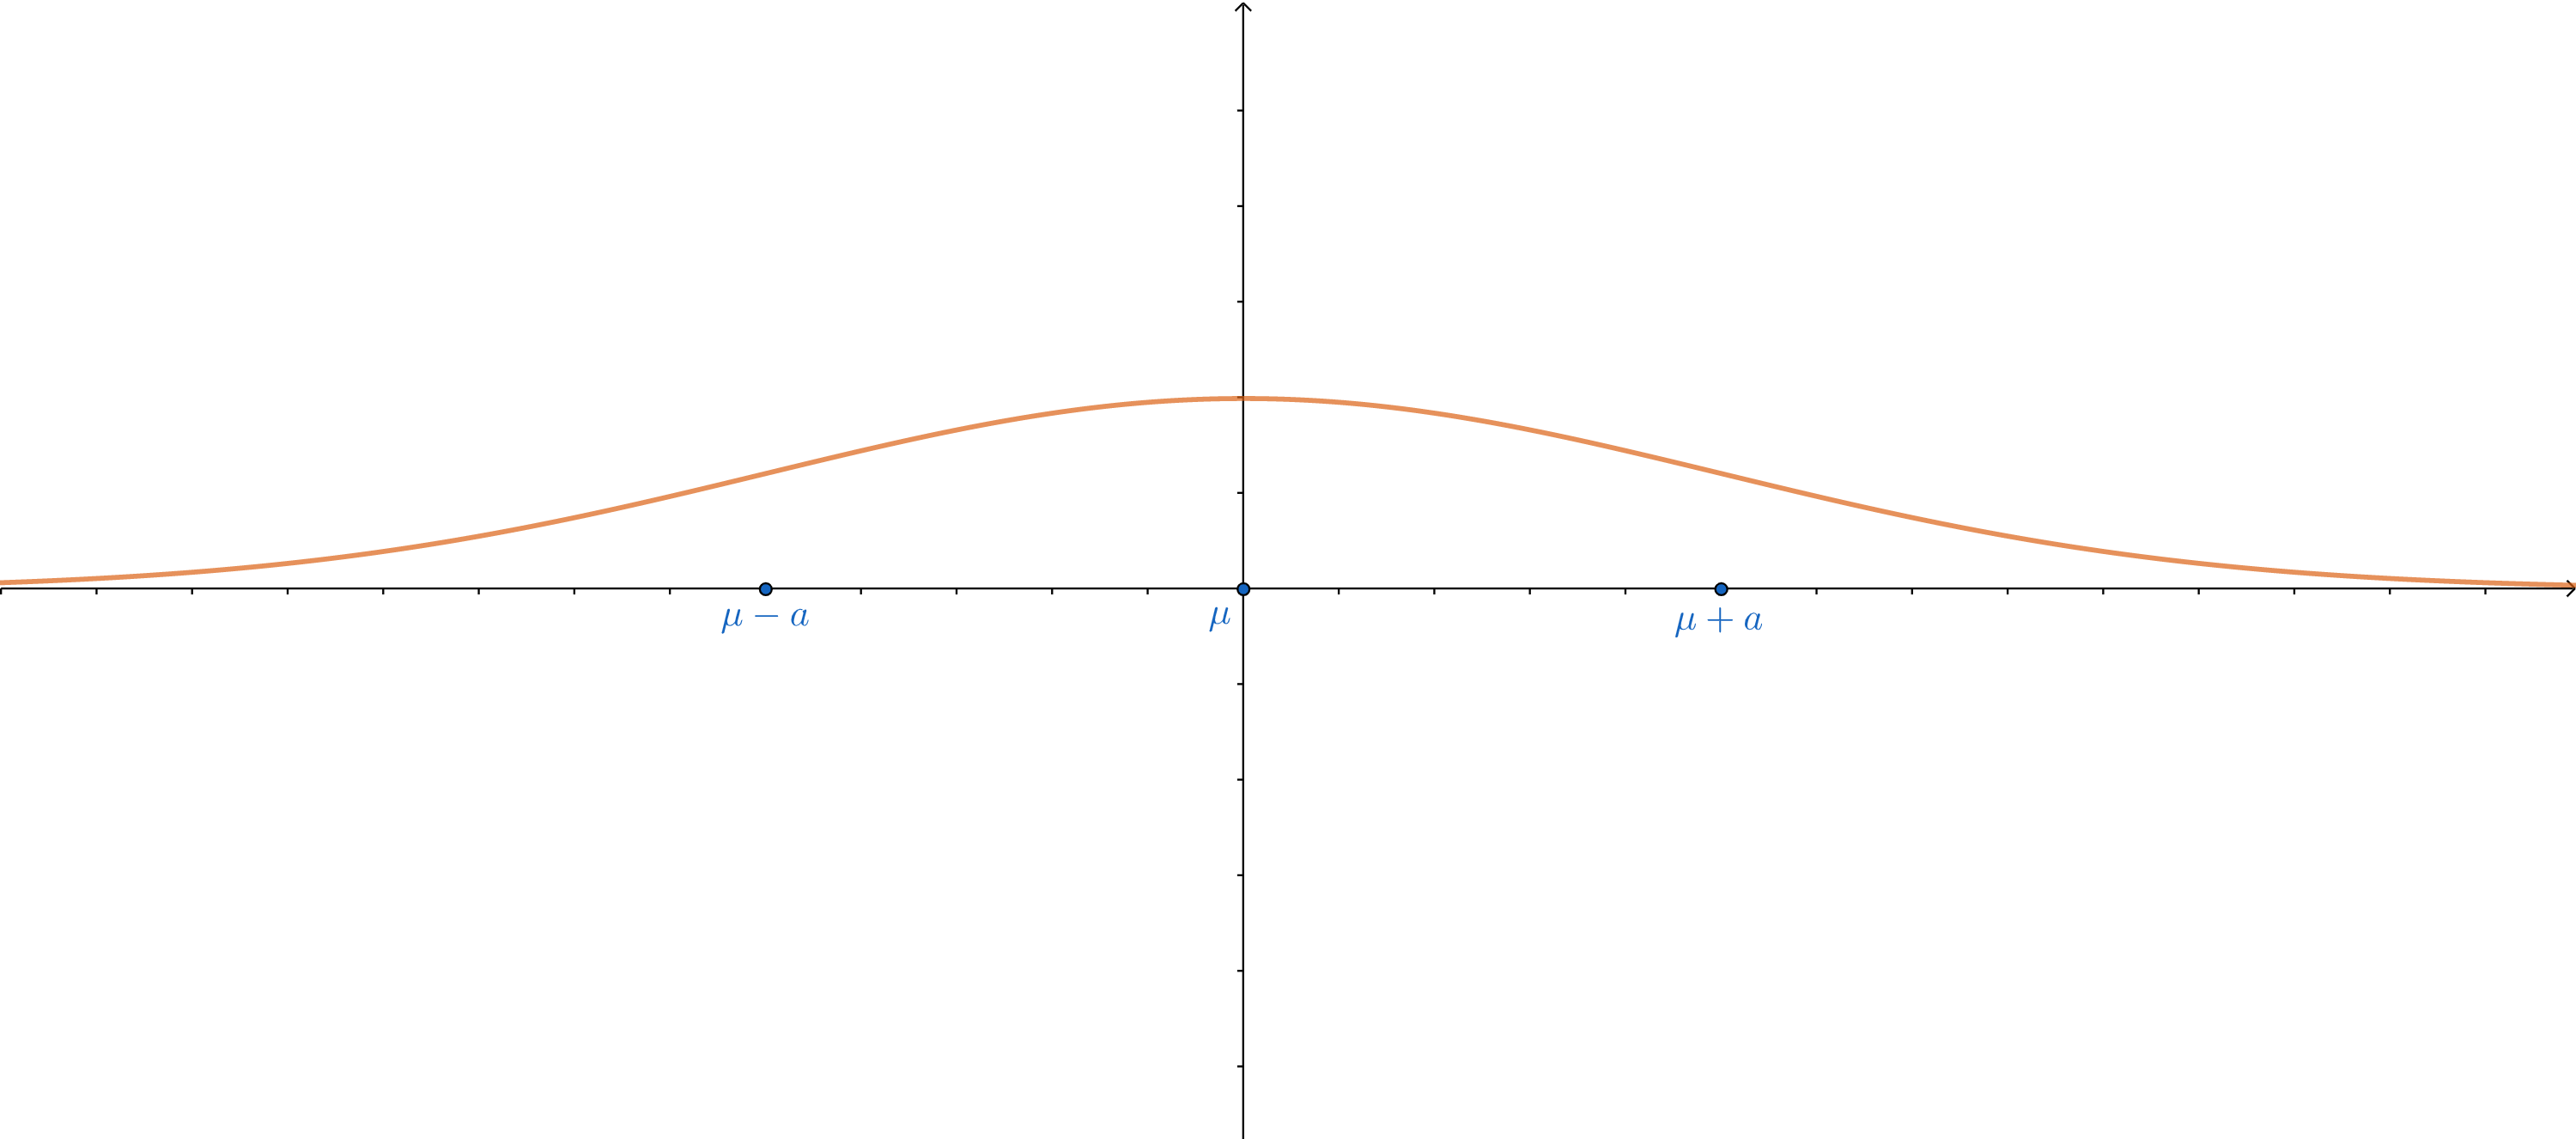
\includegraphics[width=\textwidth]{Imagens/p110.png}
    \caption{Gráfico obtido de \cite{Hoel}.}
%    \label{fig:my_label}
\end{figure}
As variáveis aleatórios com distribuição normal ocorrem frequentemente em aplicações práticas. A Lei de Maxwell da Física afirma que, sob condições adequadas, as componentes da velocidade de uma molécula de gás estarão aleatoriamente distribuídas seguindo uma distribuição normal $N(0,\sigma^2)$, onde $\sigma^2$ depende de certas quantidades físicas. Entretanto, na maioria das aplicações, as v.a.'s de interesse têm distribuições que é \textbf{aproximadamente} normal. Por exemplo, erros instrumentais em experimentos físicos e variabilidade biológica (e.g., altura e massa) foram verificados, empiricamente, como possuindo distribuições aproximadamente normais. Veremos esse tipo de comportamente mais adiante.
\end{example}

\begin{example}[Gama, $X\sim\Gamma(\alpha, \lambda)$]
Dizemos que $X$ é v.a. contínua com distribuição \textbf{gama} de parâmetros $\alpha$ e $\lambda$ (positivos) se tem densidade dada por
\begin{align*}
    f(x) = \begin{cases}
    \frac{\lambda^{\alpha}}{\Gamma(\alpha)}x^{\alpha - 1}e^{-\lambda x}, x > 0 \\
    0, x\leq 0
    \end{cases}
\end{align*}
sendo
\begin{align*}
    \Gamma(\alpha) = \int_{0}^{\infty} x^{\alpha - 1}e^{-x} dx, \alpha > 0
\end{align*}
a \textbf{função gama}. Em particular, pode-se mostrar que $\Gamma(\alpha) \in\mathbb{R}^*_+$ para todo $\alpha$ real positivo, apesar de não haver uma forma fechada para a integral. Verificamos que $f$ é densidade.
\begin{proof}
É imediato que $f(x)\geq 0, \forall x\in\mathbb{R}$. Ademais, temos
\begin{align*}
    \int_{0}^{\infty} x^{\alpha - 1}e^{-\lambda x} dx = \int_{0}^{\infty} y^{\alpha - 1}\lambda^{1 - \alpha}e^{-y}\frac{1}{\lambda} dy = \frac{1}{\lambda^{\alpha}}\int_{0}^{\infty} y^{\alpha - 1}e^{-y} dy = \frac{\Gamma(\alpha)}{\lambda^{\alpha}},
\end{align*}
logo
\begin{align*}
    \int_{\mathbb{R}} f(x) dx = \int_{0}^{\infty} \frac{\lambda^{\alpha}}{\Gamma(\alpha)} x^{\alpha - 1}e^{-\lambda x} dx = \frac{\lambda^{\alpha}}{\Gamma(\alpha)}\frac{\Gamma(\alpha)}{\lambda^{\alpha}} = 1.
\end{align*}
\end{proof}
A função gama possui algumas propriedades, muito úteis nos cálculos:
\begin{enumerate}[(i)]
    \item $\displaystyle{ \Gamma(1) = \int_{0}^{\infty} e^{-x} dx = 1 }$
    \item $\displaystyle{ \Gamma(1/2) = \int_{0}^{\infty} \frac{e^{-x}}{\sqrt{x}} dx = \sqrt{2} \int_{0}^{\infty} e^{-t^2/2} dt = \sqrt{2}\frac{1}{2}\sqrt{2\pi} = \sqrt{\pi}}$
    \item $\displaystyle{ \Gamma(\alpha + 1) = \int_{0}^{\infty} x^{\alpha} e^{-x} dx = -x^{\alpha}e^{-x}\Big|_{0}^{\infty} + \int_{0}^{\infty} \alpha x^{\alpha - 1} e^{-x} dx = \alpha\Gamma(\alpha)}$
    \item $\Gamma(1) = 1$ e $\Gamma(\alpha + 1) = \alpha\Gamma(\alpha)$ implicam $\Gamma(n) = (n-1)!, \forall n\in\mathbb{N}$
    \item $\Gamma(\alpha + 1) = \alpha\Gamma(\alpha)$ e $\Gamma(1/2) = \sqrt{\pi}$ implicam
    \begin{align*}
        \Gamma(n/2) = \frac{ \sqrt{\pi} }{ 2^{\frac{n-1}{2}} } \prod_{j=1}^{\frac{n-1}{2}} (n-2j) = \frac{ \sqrt{\pi} }{ 2^{\frac{n-1}{2}} }\frac{1}{2^{\frac{n-1}{2}}}\frac{(n-1)!}{\left( \frac{n-1}{2} \right)!} = \frac{ \sqrt{\pi} }{ 2^{n-1} }\frac{(n-1)!}{\left( \frac{n-1}{2} \right)!}, \forall n\in\mathbb{N} \text{ ímpar.}
    \end{align*}
    \item $X\sim\text{Exp}(\lambda)\iff X\sim\Gamma(1, \lambda)$, ou seja, a distribuição exponencial é um caso particular da distribuição gama
    \item se $\alpha = m \in\mathbb{N}$ com $m\geq 2$, então a f.d. $F$ de $X\sim\Gamma(m,\lambda)$ tem uma forma fechada:
    \begin{align*}
        \int_{0}^x \frac{ \lambda^m y^{m-1} e^{-\lambda y} }{(m-1)!} dy &= \frac{ -(\lambda y)^{m-1} e^{-\lambda y} }{(m-1)!}\Big|_{0}^{x} + \int_{0}^x \frac{ \lambda^{m-1} y^{m-2} e^{-\lambda y} }{ (m-2)! } dy \\
        &= \int_{0}^x \frac{ \lambda^{m-1} y^{m-2} e^{-\lambda y} }{ (m-2)! } dy - \frac{ (\lambda x)^{m-1} e^{-\lambda x} }{(m-1)!} \\
        &\vdots \\
        &= 1 - \sum_{k=0}^{m-1} \frac{ (\lambda x)^k }{k!}e^{-\lambda x}, x>0,
    \end{align*}
    em que integramos por partes $m$ vezes. Isso sugere uma conexão com $Y\sim\text{Poisson}(\lambda x)$. De fato, segue do fato acima que $P(X\leq x) = P(Y\geq m)$, e essa conexão tem aplicações em processos de Poisson.
\end{enumerate}
\end{example}

\begin{remark}[Construção de funções de densidade]
Seja $g:\mathbb{R}\to\mathbb{R}$ uma função tal que $g(x)\geq 0, \forall x\in\mathbb{R}$ e $\displaystyle{ \int_{\mathbb{R}} g(x) dx = c\in\mathbb{R}^{*}_{+} }$. Logo, se $f(x) := g(x)/c, \forall x\in\mathbb{R}$, então $f$ é densidade.
\begin{example}
Seja $g(x) = \displaystyle{ \frac{1}{1+x^2}, x\in\mathbb{R} }$. Temos $g(x)\geq 0, \forall x\in\mathbb{R}$ e 
\begin{align*}
    \int_{\mathbb{R}} g(x) dx = \lim_{a\to +\infty} \left[ \arctan x \Big|_{-a}^{a} \right] = \pi\in\mathbb{R}^*_+.
\end{align*}
Logo, $f(x) = \displaystyle{ \frac{1}{\pi(1 + x^2)} }$ é densidade.
\end{example}
\end{remark}

\begin{example}[Cauchy padrão, $X\sim\text{Cauchy}(0,1)$]
Dizemos que $X$ é v.a. contínua com distribuição \textbf{Cauchy} de parâmetros 0 e 1 se tem densidade dada por
\begin{align*}
    f(x) = \frac{1}{\pi(1+x^2)}, \forall x\in\mathbb{R}.
\end{align*}
A f.d. $F$ associada a $f$ é dada por
\begin{align*}
    F(x) = \int_{-\infty}^x f(t) dt = \frac{1}{\pi}\arctan t\Big|_{-\infty}^{x} = \frac{1}{2} + \frac{1}{\pi}\arctan x, \forall x\in\mathbb{R}.
\end{align*}
Podemos considerar também $X\sim\text{Cauchy}(\mu, \beta)$, com $\mu$ real e $\beta$ real positivo, chamada \textbf{distribuição Cauchy} de parâmetros $\mu$ e $\beta$. Essa v.a. tem densidade dada por
\begin{align*}
    f(x) = \frac{\beta}{\pi(\beta^2 + (x-\mu)^2)}, \forall x\in\mathbb{R}.
\end{align*}
Verificamos que $f$ é densidade.
\begin{proof}
Note que $f(x) \geq 0, \forall x\in\mathbb{R}$ e que
\begin{align*}
    \int_{\mathbb{R}} f(x) dx = \frac{1}{\pi}\int_{-\infty}^{\infty} \frac{1}{\beta}\cdot\frac{ 1 }{ 1 + \left( \frac{x-\mu}{\beta} \right)^2 } dx = \frac{1}{\pi}\int_{-\infty}^{\infty} \frac{1}{1+y^2} dy = 1.
\end{align*}
\end{proof}
\end{example}

\subsection{Funções de variáveis aleatórias contínuas}
Sendo $X$ v.a. contínua e $g$ função em $\mathbb{R}$, estamos interessados em determinar a densidade $f_Y$ de $Y = g(X)$.

\begin{example}
Seja $Y = X^2$, i.e., $Y = g(X)$ com $g:\mathbb{R}\to\mathbb{R}$ tal que $g(x) = x^2$. Note que se $y\leq 0$, então $F_Y(y) = P(Y\leq y) = 0$ e, se $y>0$, então $F_Y(y) = P(Y\leq y) = P(X^2\leq y) = P(-\sqrt{y} \leq X\leq \sqrt{y}) = F_X(\sqrt{y}) - F_X(-\sqrt{y})$. Logo, segue que para $y>0$ temos
\begin{align*}
    f_Y(y) = F_X'(\sqrt{y})\frac{d}{dy}(\sqrt{y}) - F_X'(-\sqrt{y})\frac{d}{dy}(-\sqrt{y}) = \frac{1}{2\sqrt{y}}[f_X(\sqrt{y}) + f_X(-\sqrt{y})],
\end{align*}
ou seja, 
\begin{align*}
    f_Y(y) = \begin{cases}
    \frac{1}{2\sqrt{y}}[f_X(\sqrt{y}) + f_X(-\sqrt{y})], y > 0 \\
    0, y\leq 0
    \end{cases}.
\end{align*}
Essa fórmula vale para todo $y$ onde $F_X'(\sqrt{y})$ existe.
\end{example}

\begin{remark}
Se $X$ é v.a. contínua com densidade $f_X$ e $g$ é uma função discreta, i.e., com imagem finita ou enumerável, então $Y=g(X)$ é v.a. discreta.
\end{remark}

\begin{example}
Se $X\sim\text{Exp}(1)$ e $Y = I_{X\leq 3}$, i.e.,
\begin{align*}
    Y = g(X) = \begin{cases}
    1, X\leq 3 \\
    0, X > 3
    \end{cases},
\end{align*}
então os valores possíveis de $Y$ são 0 e 1. Temos $P(Y=1) = P(X\leq 3) = 1 - e^{-3}$, $P(Y=0) = P(X>3) = e^{-3}$ e $P(Y=y) = 0, \forall y\in\mathbb{R}\setminus\{0,1\}$. Logo,
\begin{align*}
    p_Y(y) = \begin{cases}
    e^{-3}, y = 0 \\
    1 - e^{-3}, y = 1 \\
    0, \text{ c.c.}
    \end{cases}
\end{align*}
é a f.p. de $Y$ (discreta!).
\end{example}

\begin{theorem}[Mudança de variável]
Seja $X$ v.a. contínua com f.d. $f_X$ tal que $f_X(x) = 0$ para todo $x\in I$, sendo $I$ um aberto da reta. Suponha que $g:\mathbb{R}\to\mathbb{R}$ seja uma função estritamente monótona e derivável em $I$. Então $Y=g(X)$ tem densidade dada por
\begin{align*}
    f_Y(y) = \begin{cases}
    f_x(g^{-1}(y))\left| \frac{d}{dy}g^{-1}(y) \right|, y\in g(I) \\
    0, y\notin g(I)
    \end{cases}.
\end{align*}
Podemos simplificar a notação tomando $x = g^{-1}(y)$.
\end{theorem}

\begin{proof}
Note que $g$ é derivável e inversível em $I$. Suponhamos $g$ estritamente crescente em $I$. Então $g^{-1}$ é estritamente crescente em $g(I)$. Daí, dado $y\in g(I)$, temos
\begin{align*}
    F_Y(y) = P(Y\leq y) = P(g(X)\leq y) = P(X\leq g^{-1}(y)) = F_X(g^{-1}(y)).
\end{align*}
Logo,
\begin{align*}
    f_Y(y) = \frac{d}{dy}\left[ F_X(g^{-1}(y)) \right] = f_X(g^{-1}(y))\underbrace{\frac{d}{dy}(g^{-1}(y))}_{>0},
\end{align*}
ou seja, temos
\begin{align*}
    f_Y(y) = f_x(g^{-1}(y))\left| \frac{d}{dy}g^{-1}(y)\right|.
\end{align*}
Se $g$ é estritamente decrescente em $I$, então $g^{-1}$ também o é e, dado $y\in g(I)$, temos
\begin{align*}
    F_Y(y) = P(Y\leq y) = P(g(X)\leq y) = P(X\geq g^{-1}(y)) = 1 - F_X(g^{-1}(y)).
\end{align*}
Logo,
\begin{align*}
    f_Y(y) = \frac{d}{dy}\left[1 - F_X(g^{-1}(y)) \right] = f_X(g^{-1}(y))\underbrace{\frac{d}{dy}(-g^{-1}(y))}_{>0},
\end{align*}
ou seja, temos
\begin{align*}
    f_Y(y) = f_x(g^{-1}(y))\left| \frac{d}{dy}g^{-1}(y)\right|.
\end{align*}
\end{proof}

\begin{example}
Sejam $X\sim\text{Exp}(\lambda)$ e $Y = X^{1/\beta}, \beta\in\mathbb{R}^*$. Temos
\begin{align*}
    f_X(x) = \begin{cases}
    \lambda e^{-\lambda x}, x > 0 \\
    0, x\leq 0
    \end{cases}.
\end{align*}
Ademais, $Y = g(X)$ com $g$ função da reta dada por $g(x) = x^{1/\beta}$. Note que $g$ é crescente e derivável em $(0, +\infty)$ e também
\begin{align*}
    y = x^{1/\beta} \iff x = y^{\beta} \implies \frac{dx}{dy} = \beta y^{\beta - 1}.
\end{align*}
Daí, se $y>0$, temos
\begin{align*}
    f_Y(y) = f_X(x)\left|\frac{dx}{dy}\right| = \lambda e^{-\lambda y^{\beta}}|\beta y^{\beta -1}|
\end{align*}
e, portanto,
\begin{align*}
    f_Y(y) = \begin{cases}
    \lambda |\beta| y^{\beta - 1}e^{-\lambda y^{\beta}}, y> 0 \\
    0, y\leq 0.
    \end{cases}
\end{align*}
\end{example}

\begin{example}
Sejam $X$ v.a. contínua com densidade $f_X$ e $a,b\in\mathbb{R}$ com $b\neq 0$. Se $Y = a + bX$, então
\begin{align*}
    y = a + bx \iff x = \frac{y-a}{b} \implies \frac{dx}{dy} = \frac{1}{b},
\end{align*}
com $g$ função da reta dada por $g(x) = a + bx$ estritamente monótona em $\mathbb{R}$ (que é um aberto). Logo, dadao $y\in\mathbb{R}$, temos
\begin{align*}
    f_Y(y) = f_X\left( \frac{y-a}{b} \right)\left|\frac{1}{b}\right|.
\end{align*}
\end{example}

\begin{proposition}
Sejam $X$ v.a. contínua e $\mu, \sigma\in\mathbb{R}$ com $\sigma > 0$. Temos
\begin{enumerate}[(i)]
    \item se $Y = \displaystyle{ \frac{X-\mu}{\sigma} }$, então $X\sim N(\mu, \sigma^2) \iff Y\sim N(0,1)$
    \item se $X\sim N(\mu, \sigma^2)$ e $Y = a + bX$ com $a,b\in\mathbb{R}$ e $b\neq 0$, então $Y\sim N(a+b\mu, b^2\sigma^2)$
    \item se $X\sim N(0,1)$ e $Y=-X$, então $Y\sim N(0,1)$
\end{enumerate}
\end{proposition}

\begin{proof}
\begin{enumerate}[(i)]
    \item Note que $g:\mathbb{R}\to\mathbb{R}$ dada por $g(x) = \displaystyle{ \frac{x-\mu}{\sigma} }$ é estritamente crescente e derivável na reta. Daí, temos
    \begin{align*}
        x = \sigma y + \mu \implies \frac{dx}{dy} = \sigma.
    \end{align*}
    Logo, 
    \begin{align*}
        f_Y(y) = \frac{1}{\sqrt{2\pi}\sigma}e^{ -\frac{(y-\mu)^2}{2\sigma^2} }\sigma = \frac{1}{\sqrt{2\pi}}e^{-y^2/2}, y\in\mathbb{R},
    \end{align*}
    ou seja, $Y\sim N(0,1)$. Reciprocamente, se $Y\sim N(0,1)$ então
    \begin{align*}
        f_X(x) = f_Y(g(x))\left|\frac{dy}{dx}\right| = \frac{1}{\sqrt{2\pi}\sigma}\exp[-\frac{1}{2}(\frac{x-\mu}{\sigma})^2]
    \end{align*}
    ou seja, $X\sim N(\mu, \sigma^2)$.
    \item Utilizando o exemplo anterior, temos
    \begin{align*}
        f_Y(y) = f_X(g^{-1}(y))\left|\frac{dx}{dy}\right| = \frac{1}{\sqrt{2\pi}\sigma}\exp[-\frac{1}{2}\frac{1}{\sigma^2}(\frac{y-a}{b} - \mu)^2]\left|\frac{1}{b}\right| = \frac{1}{\sqrt{2\pi}\sigma|b|} \exp[ -\frac{1}{2}\frac{ [ y - (a+b\mu) ]^2 }{ (\sigma b)^2 } ],
    \end{align*}
    ou seja, $Y\sim N(a + b\mu, b^2\sigma^2)$.
    \item Note que $g:\mathbb{R}\to\mathbb{R}$ dada por $g(x) = -x$ é estritamente decrescente e derivável em $\mathbb{R}$. Ademais, temos $x = -y$ e $dx/dy = -1$, de modo que
    \begin{align*}
        f_Y(y) = f_X(g^{-1}(y)) \left|\frac{dx}{dy}\right| = \frac{1}{\sqrt{2\pi}}\exp[ -\frac{1}{2}(-y)^2 ]|-1| = \frac{1}{\sqrt{2\pi}} e^{-y^2/2},
    \end{align*}
    ou seja, $Y\sim N(0,1)$.
\end{enumerate}
\end{proof}

\section{Vetores aleatórios contínuos}
Começamos com as definições gerais, generalizando de maneira natural as definições vistas na seção anterior.

\subsection{Definições gerais}
\begin{definition}[Vetor aleatório]
Sejam $X_1, X_2, \dots, X_n$ v.a.'s absolutamente contínuas, definidas em $(\Omega, \mathcal{A}, P)$. Chamamos $\overline{X} = (X_1, \dots, X_n)$ de \textbf{vetor aleatório contínuo} ($n$-dimensional).

Dito de outro modo, $\overline{X}$ é vetor aleatório contínuo se sua função de distribuição $F_{X_1, \dots, X_n}$ é dada por
\begin{align*}
    F_{\overline{X}}(\overline{x}) = P(X_1\leq x_1, \dots, X_n\leq x_n) = \int_{-\infty}^{x_1}\cdots\int_{-\infty}^{x_n} f(u_1, \dots, u_n) du_n\cdots du_1, \forall \overline{x}\in\mathbb{R}^n,
\end{align*}
para alguma função $f:\mathbb{R}^n\to\mathbb{R}$ função de densidade $n$-dimensional, isto é, $f(\overline{x}) \geq 0 \forall\overline{x}\in\mathbb{R}$ e $\displaystyle{ \int_{\mathbb{R}} \cdots \int_{\mathbb{R}} f(x_1, \dots, x_n) dx_1\cdots dx_n = 1 }$. Nesse caso, dizemos que $f$ é \textbf{função de densidade} de $\overline{X}$ e denotamos $f:= f_{\overline{X}}$.
\end{definition}

\begin{definition}
Seja $F_{X_1, \dots, X_n}$ a f.d. de $(X_1, \dots, X_n)$. Para cada $k\in\{1,\dots,n\}$, definimos a \textbf{função de distribuição marginal} de $X_k$ por
\begin{align*}
    F_{X_k}(x_k) = P(X_k\leq x_k) = \lim_{x_i\to +\infty, i\neq k} F_{X_1, \dots, X_n}(x_1, \dots, x_n), x_k\in\mathbb{R}.
\end{align*}
Podemos definir a f.d. marginal de pares, triplas e $r$-uplas de maneira inteiramente análoga.
\end{definition}

\subsection{Distribuições marginais e independência}
\paragraph{Caso bidimensional.} Seja $(X,Y)$ um vetor aleatório contínuo com densidade conjunta $f = f_{X,Y}$ e f.d. conjunta $F = F_{X,Y}$. Temos
\begin{align*}
    F(x,y) = P(X\leq x, Y\leq y) = \int_{-\infty}^x\int_{-\infty}^y f(u,v) dvdu, \forall (x,y)\in\mathbb{R}^2
\end{align*}
e também
\begin{align*}
    P(a < X\leq b, c < Y\leq d) = \int_{a}^{b}\int_{c}^{d} f(x,y) dydx.
\end{align*}
De maneira geral, 
\begin{align*}
    P((X,Y)\in A) = \iint_A f(x,y) dxdy, \forall A\in\mathcal{B}^2(\mathbb{R}).
\end{align*}
Podemos, ainda, obter as densidades marginais de $X$ e $Y$. Note que
\begin{align*}
    F_X(x) = P(X\leq x) = P(X\leq x, Y\in\mathbb{R}) = \int_{-\infty}^{x}\int_{-\infty}^{\infty} f(u,y) dydu.
\end{align*}
Por outro lado, sabemos que
\begin{align*}
    F_X(x) = \int_{-\infty}^{x} f_X(u) du.
\end{align*}
Logo, como ambas as igualdades valem para todo $x\in\mathbb{R}$, devemos ter
\begin{align*}
    f_X(x) = \int_{-\infty}^{\infty} f_{X,Y}(x,y) dy, \forall x\in\mathbb{R}.
\end{align*}
De maneira análoga, temos
\begin{align*}
    F_Y(y) = \int_{-\infty}^{y}\int_{-\infty}^{\infty} f(x,v) dxdv
\end{align*}
e
\begin{align*}
    f_Y(y) = \int_{-\infty}^{\infty} f_{X,Y}(x,y) dx, \forall y\in\mathbb{R}.
\end{align*}
Sob algumas fracas condições de regularidades e para $(x,y)$ ponto de continuidade de $f$, temos
\begin{align*}
    \frac{\partial}{\partial y}F(x,y) = \int_{-\infty}^x \left( \frac{\partial}{\partial y} \int_{-\infty}^y f(u,v) dv \right) du = \int_{-\infty}^x f(u,y) du,
\end{align*}
de modo que
\begin{align*}
    \frac{\partial^2}{\partial x\partial y}F(x,y) = f(x,y)
\end{align*}
e também, de maneira análoga,
\begin{align*}
    \frac{\partial^2}{\partial y\partial x}F(x,y) = f(x,y).
\end{align*}

\begin{example}
Sejam $X, Y$ v.a.'s contínuas com f.d. conjunta $F$ dada por
\begin{align*}
    F(x,y) = \begin{cases}
    0, x<0 \text{ e } y<0 \\
    \frac{x}{5}(1 - e^{-y}), 0\leq x\leq 5 \text{ e } y\geq 0 \\
    1 - e^{-y}, x\geq 5 \text{ e } y\geq 0
    \end{cases}.
\end{align*}
Note que
\begin{align*}
    F_X(x) = \lim_{y\to\infty} F(x,y) = \begin{cases}
    0, x < 0 \\
    x/5, 0\leq x < 5 \\
    1, x\geq 5
    \end{cases}
\end{align*}
e também
\begin{align*}
    F_Y(y) = \lim_{x\to\infty} F(x,y) = \begin{cases}
    0, y < 0 \\
    1 - e^{-y}, y\geq 0
    \end{cases}.
\end{align*}
Ademais, para todo $(x,y)\in\mathbb{R}^2$ com $x\notin\{0,5\}$ e $y\neq 0$, temos
\begin{align*}
    \frac{\partial}{\partial y}F(x,y) = \begin{cases}
    0, x < 0 \text{ e } y < 0 \\
    \frac{x}{5}e^{-y}, 0 < x < 5 \text{ e } y > 0 \\
    e^{-y}, x > 5 \text{ e } y>0
    \end{cases}
\end{align*}
e também
\begin{align*}
    \frac{\partial^2}{\partial x\partial y}F(x,y) = \begin{cases}
    0, x < 0 \text{ e } y < 0 \\
    \frac{e^{-y}}{5}, 0 < x < 5 \text{ e } y > 0 \\
    0, x > 5 \text{ e } y>0
    \end{cases}.
\end{align*}
Portanto, 
\begin{align*}
    f_{X,Y}(x,y) = \begin{cases}
    e^{-y}/5, 0 < x < 5 \text{ e } y > 0 \\
    0, \text{ c.c.}
    \end{cases}
\end{align*}
e obtemos
\begin{align*}
    f_X(x) &= \frac{d}{dx}F_X(x) = \begin{cases}
    1/5, 0 < x < 5 \\
    0, \text{ c.c.}
    \end{cases} \\
    f_Y(y) &= \frac{d}{dy}F_Y(y) = \begin{cases}
    e^{-y}, y > 0 \\
    0, \text{ c.c.}
    \end{cases},
\end{align*}
ou seja, $X\sim U(0,5)$ e $Y\sim\text{Exp}(1)$.
\end{example}

\begin{example}
Seja $D = \{ (x,y)\in\mathbb{R}^2 : x^2+y^2\leq R^2 \}$ e considere o experimento de escolher um ponto em $D$. Defina $X$ e $Y$ como as coordenadas do ponto escolhido. Supondo uniformidade, temos que a densidade conjunta de $X$ e $Y$ é dada por
\begin{align*}
    f(x,y) = \begin{cases}
    \frac{1}{\pi R^2}, (x,y)\in D \\
    0, \text{ c.c.}
    \end{cases}.
\end{align*}
De fato, note que dado $A\subset D$ temos
\begin{align*}
    P((X,Y)\in A) = \iint_A f(x,y) dxdy.
\end{align*}
Da hipótese de uniformidade, temos
\begin{align*}
    P((X,Y)\in A) = \frac{ \iint_A dxdy }{ \pi R^2 } = \iint_A \frac{1}{\pi R^2} dxdy,
\end{align*}
de modo que $f$ tem a forma acima. Para as densidades marginais, temos que dado $-R < x < R$,
\begin{align*}
    f_X(x) = \int_{\mathbb{R}} f(x,y)dy = \int_{-\sqrt{R^2-x^2}}^{\sqrt{R^2-x^2}} \frac{1}{\pi R^2} dy = 2\frac{\sqrt{R^2 - x^2}}{\pi R^2}.
\end{align*}
Logo,
\begin{align*}
    f_X(x) = \begin{cases}
    2\frac{\sqrt{R^2 - x^2}}{\pi R^2}, -R < x < R \\
    0, \text{ c.c.}
    \end{cases}
\end{align*}
e, de maneira análoga,
\begin{align*}
    f_Y(y) = \begin{cases}
    2\frac{\sqrt{R^2 - y^2}}{\pi R^2}, -R < y < R \\
    0, \text{ c.c.}
    \end{cases}
\end{align*}
\begin{figure}[H]
    \centering
    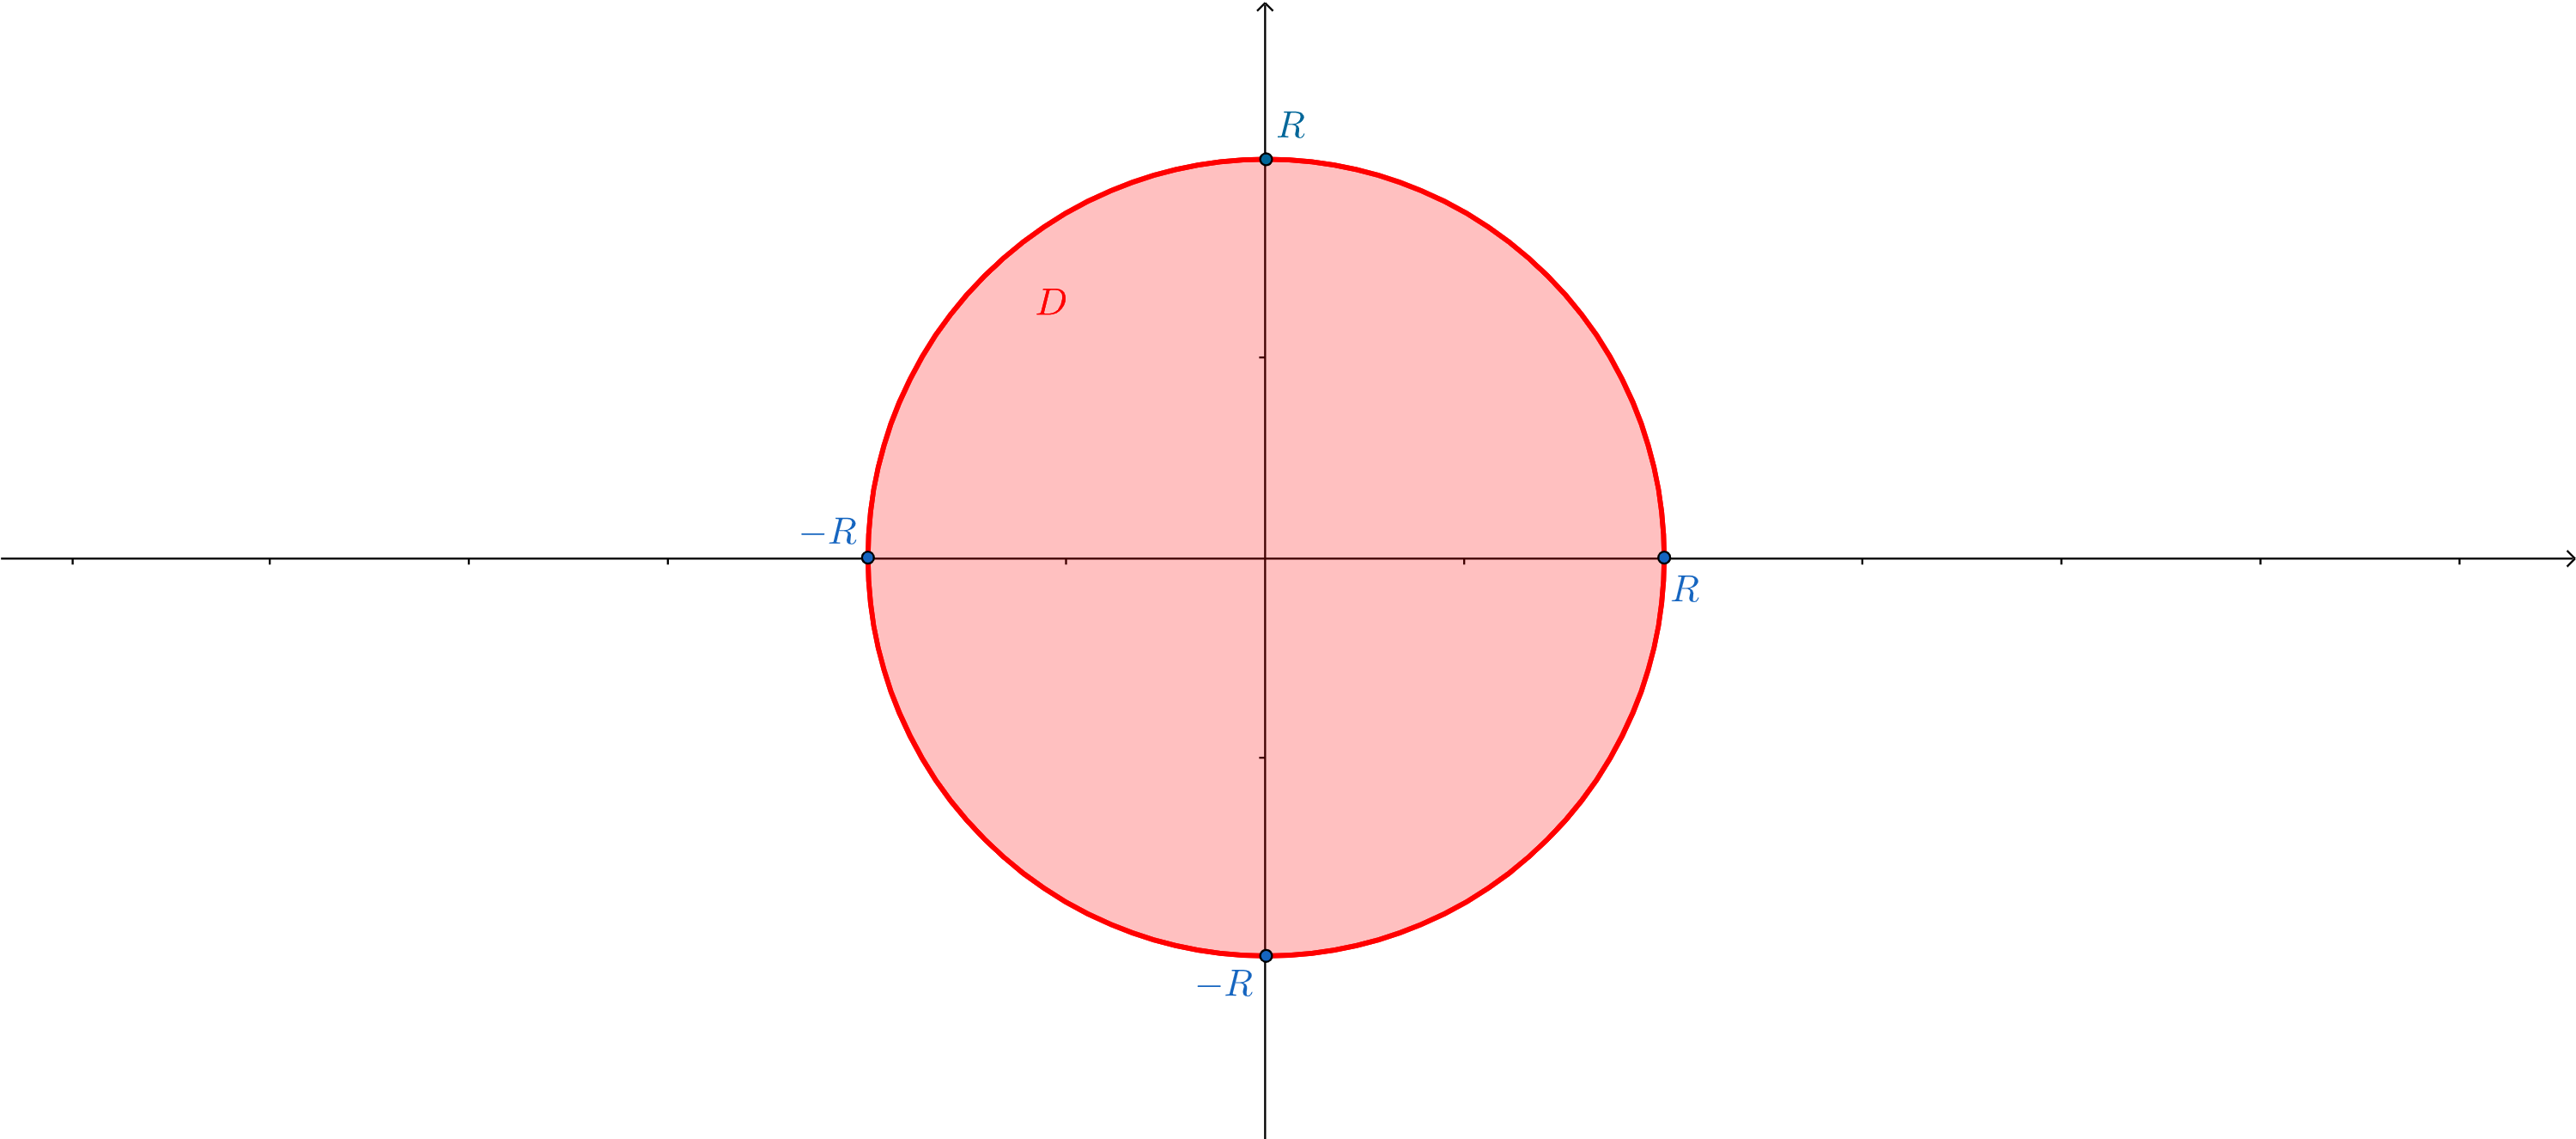
\includegraphics[width=\textwidth]{Imagens/p121.png}
    \caption{Gráfico da região $D$.}
%    \label{fig:my_label}
\end{figure}
\end{example}

Queremos agora discutir sobre a independência de duas v.a.'s contínuas. Recorde que duas v.a.'s $X$ e $Y$ são ditas independentes se estão definidas no mesmo espaço $(\Omega, \mathcal, P)$ e, dados quaisquer $A_1, A_2\in\mathcal{B}(\Omega)$, vale $P(X\in A_1, Y\in A_2) = P(X\in A_1)P(Y\in A_2)$. Vimos anteriormente que $X$ e $Y$ são v.a.'s independentes se, e só se, $F(x,y) = F_X(x)F_Y(y), \forall (x,y)\in\mathbb{R}^2$. Um resultado análogo vale para a densidade.
\begin{proposition}
Duas v.a.'s contínuas $X$ e $Y$ definidas em $(\Omega, \mathcal{A}, P)$ são independentes se, e só se, $f_{X,Y}(x,y) = f_X(x)f_Y(y), \forall (x,y)\in\mathbb{R}^2$.
\end{proposition}
\begin{proof}
Dado $(x,y)\in\mathbb{R}^2$, temos $X$ e $Y$ independentes se, e só se,
\begin{align*}
    \int_{-\infty}^{x}\int_{-\infty}^{y} f_{X,Y}(u,v) dvdu &= F_{X,Y}(x,y) \\
    &= F_X(x)F_Y(y) \\
    &= \left( \int_{-\infty}^{x} f_X(u) du \right)\left( \int_{-\infty}^{y} f_Y(v) dv \right) \\
    &= \int_{-\infty}^{x}\int_{-\infty}^{y} f_X(u)f_Y(v) dvdu.
\end{align*}
Como $(x,y)$ é um ponto arbitrário do plano, devemos ter
\begin{align*}
    f_{X,Y}(x,y) = f_X(x)f_Y(y), \forall (x,y)\in\mathbb{R}^2.
\end{align*}
\end{proof}

\begin{example}
No dois exemplos anteriores temos $X$ e $Y$ independentes no primeiro mas não no segundo.
\end{example}

\begin{example}[Construção de densidade conjunta]
Suponha $X$ e $Y$ v.a.'s i.i.d. com $X\sim N(0,1)$. Então temos
\begin{align*}
    f(x,y) = f_X(x)f_Y(y) = \frac{1}{2\pi}\exp[-\frac{x^2+y^2}{2}], \forall (x,y)\in\mathbb{R}^2.
\end{align*}
Pode-se verificar, de maneira análoga à densidade da distribuição normal, que esta $f$ define uma densidade; ela é chamada \textbf{densidade normal bidimensional padrão}.
\end{example}

\begin{example}
Sejam $X$ e $Y$ v.a.'s com densidade conjunta dada por $f(x,y) = \displaystyle{c\exp[-\frac{x^2 - xy + y^2}{2}], \forall (x,y)\in\mathbb{R}^2}$, com $c$ real positivo tal que $\displaystyle{ \iint_{\mathbb{R}^2} f(x,y)dxdy = 1 }$. Note que esta última integral é complicada de calcular diretamente. Portanto, tomamos uma rota alternativa para encontrar $c$. Note que
\begin{align*}
    f(x,y) = c\exp[ -\frac{1}{2}\left( \left(y - \frac{x}{2}\right)^2 + \frac{3}{4}x^2 \right) ].
\end{align*}
Daí, segue que
\begin{align*}
    f_X(x) = \int_{\mathbb{R}} f(x,y)dy = ce^{-3x^2/8}\int_{\mathbb{R}} \exp[ -\frac{1}{2}\left( y - \frac{x}{2} \right)^2 ]dy = ce^{-3x^2/8}\int_{\mathbb{R}} e^{-u^2/2} du = c\sqrt{2\pi}e^{-3x^2/8}, \forall x\in\mathbb{R}.
\end{align*}
Ora, mas $c$ deve ser tal que $\displaystyle{ \int_{\mathbb{R}} f_X(x) dx = 1 }$, logo
\begin{align*}
    c\sqrt{2\pi}\int_{\mathbb{R}} e^{-3x^2/8} dx = 1 \implies c\sqrt{2\pi}\frac{2}{\sqrt{3}}\int_{\mathbb{R}} e^{-u^2/2} du = 1 \implies c = \frac{\sqrt{3}}{4\pi}.
\end{align*}
Logo,
\begin{align*}
    f(x,y) = \displaystyle{\frac{\sqrt{3}}{4\pi}\exp[-\frac{x^2 - xy + y^2}{2}], \forall (x,y)\in\mathbb{R}^2}   
\end{align*}
e $X\sim N(0, 4/3)$. De maneira análoga, $Y\sim N(0, 4/3)$ e observamos que $X$ e $Y$ não são independentes, pois
\begin{align*}
    \frac{3}{8\pi} = f_X(0)f_Y(0) \neq f(0,0) = \frac{\sqrt{3}}{4\pi}.
\end{align*}
\end{example}

\paragraph{Caso $n$-dimensional.} Considere $(X_1, \dots, X_n)$ um vetor aleatório contínuo com densidade $f = f_{X_1, \dots, X_n}$ e f.d. $F = F_{X_1, \dots, X_n}$. As distribuições marginais são dadas por
\begin{align*}
    f_{X_k}(x_k) = \int_{-\infty}^{\infty}\cdots\int_{-\infty}^{\infty} f(x_1, \dots, x_n) dx_1\cdots dx_{k-1}dx_{k+1}\cdots dx_n
\end{align*}
e analogamente para os demais casos. Ademais,
\begin{align*}
    F_{X_k}(x_k) = \int_{-\infty}^{x_k} f_{X_k}(u) du = \int_{-\infty}^{x_k}\int_{-\infty}^{\infty}\cdots\int_{-\infty}^{\infty} f(x_1, \dots, x_{k-1}, u, x_{k+1}, \dots, x_n) dx_1\cdots dx_{k-1}dx_{k+1}\cdots dx_ndu
\end{align*}
e analogamente para os demais casos. De maneira geral, se $A\in\mathcal{B}^n(\mathbb{R})$ então
\begin{align*}
    P((X_1, \dots, X_n)\in A) = \int \cdots \int_A f(x_1, \dots, x_n) dx_1\cdots dx_n.
\end{align*}
Novamente sob algumas condições fracas de regularidade, podemos escrever
\begin{align*}
    f(x_1, \dots, x_n) = \frac{\partial^n}{\partial x_1\cdots\partial x_n}F(x_1, \dots, x_n), \forall (x_1, \dots, x_n)\in\mathbb{R}^n \text{ tal que } f \text{ é contínua.}
\end{align*}
Naturalmente, $X_1, \dots, X_n$ são independentes se, e só se, $F(x_1, \dots, x_n) = F_{X_1}(x_1)\cdots F_{X_n}(x_n), \forall (x_1, \dots, x_n)\in\mathbb{R}^n$ ou, equivalentemente, se, e só se, $f(x_1, \dots, x_n) = f_{X_1}(x_1)\cdots f_{X_n}(x_n), \forall (x_1, \dots, x_n)\in\mathbb{R}^n$.

\subsection{Função de distribuição $n$-dimensional}
Dada $F:\mathbb{R}^n\to\mathbb{R}$ uma função, estamos interessados em saber as condições que $F$ deve satisfazer para ser função de distribuição em $\mathbb{R}^n$. Pensando na f.d. unidimensional, as três condições a seguir são naturais de serem exigidas.
\begin{itemize}
    \item[(F1)] $F(x_1, \dots, x_n)$ é não decrescente em cada variável, ou seja, se $x<y$ então
    \begin{align*}
        F(x_1, \dots, x_{k-1}, x, x_{k+1}, \dots, x_n) \leq F(x_1, \dots, x_{k-1}, y, x_{k+1}, \dots, x_n), \forall k\in\{1,\dots, n\}.
    \end{align*}
    \item[(F2)] $F(x_1, \dots, x_n)$ é contínua à direita em cada variável, ou seja, se $y_m\xrightarrow{m\to\infty} x_k$ então
    \begin{align*}
        F(x_1, \dots, x_{k-1}, y_m, x_{k+1}, \dots, x_n) \xrightarrow{m\to\infty} F(x_1, \dots, x_{k-1}, x_k, x_{k+1}, \dots, x_n), \forall k\in\{1, \dots, n\}.
    \end{align*}
    \item[(F3)] Vale
    \begin{align*}
        \lim_{x_i\to -\infty} F(x_1, \dots, x_i, \dots, x_n) := F(x_1, \dots, -\infty, \dots, x_n) = 0, \forall i = 1,2, \dots, n
    \end{align*}
    e também
    \begin{align*}
        \lim_{x_1\to \infty}\cdots\lim_{x_n\to \infty} F(x_1, \dots, x_n) := F(+\infty, \dots, +\infty) = 1.
    \end{align*}
\end{itemize}
No entanto, apenas essas três condições não são suficientes. De fato, tome $F:\mathbb{R}^2\to\mathbb{R}$ tal que
\begin{align*}
    F(x,y) = \begin{cases}
    1, x\geq 0, y\geq 0 \text{ e } x+y\geq 1 \\
    0, \text{ c.c.}
    \end{cases}.
\end{align*}
Note que $F$ satisfaz as três condições acima, mas supondo que $F$ fosse f.d. de $(X,Y)$ então teríamos
\begin{align*}
    0\leq P(0 < X\leq 1, 0 < Y\leq 1) &= P(X\leq 1, 0 < Y\leq 1) - P(X\leq 0, 0 < Y\leq 1) \\
    &= F(1,1) - F(1,0) - F(0,1) + F(0,0) \\
    &= 1 - 1 - 1 + 0 \\
    &= -1,
\end{align*}
absurdo. Assim, queremos que dados $a_1 < b_1$ e $a_2 < b_2$ reais, $F$ seja tal que
\begin{align*}
    0\leq P(a_1 < X\leq b_1, a_2 < Y\leq b_2) = F(b_1, b_2) - F(b_1, a_2) - [F(a_1, b_2) - F(a_1, a_2)].
\end{align*}
De maneira geral, temos a condição
\begin{itemize}
    \item[(F4)] Se $I_k = (a_k, b_k], k = 1,2,\dots,n$ e $\Delta_{k, I_k}F(x_1, \dots, x_n)$ for definido como
    \begin{align*}
        F(x_1, \dots, x_{k-1}, b_k, x_{k+1}, \dots, x_n) - F(x_1, \dots, x_{k-1}, a_k, x_{k+1}, \dots, x_n),
    \end{align*}
    então
    \begin{align*}
        \Delta_{1, I_1}\cdots\Delta_{n,I_n}F(x_1, \dots, x_n) \geq 0, \forall I_k = (a_k,b_k], k = 1,\dots,n.
    \end{align*}
\end{itemize}
Com isso, definimos
\begin{definition}
Uma função $F:\mathbb{R}^n\to\mathbb{R}$ que satisfaz (F1), (F2), (F3) e (F4) é chamada \textbf{função de distribuição} $n$-dimensional.
\end{definition}

\begin{proposition}
Dado um vetor aleatório $(X_1, \dots, X_n)$, a função $F:\mathbb{R}^n\to\mathbb{R}$ dada por
\begin{align*}
    F_{X_1, \dots, X_n}(x_1, \dots, x_n) = P(X_1\leq x_1, \dots, X_n\leq x_n), \forall (x_1, \dots, x_n)\in\mathbb{R}^n
\end{align*}
define uma f.d. em $\mathbb{R}^n$.
\end{proposition}

\begin{proof}
Basta verificar (F1)-(F4) usando as propriedades da medida de probabilidade.
\end{proof}

\subsection{Funções de vetores aleatórios}
Sejam $(X_1, \dots, X_n)$ vetor aleatório com densidade $f_{X_1, \dots, X_n} = f$, função de distribuição $F_{X_1, \dots, X_n} = F$ e $Z = g(X_1, \dots, X_n)$, com $g:D\subset\mathbb{R}^n\to\mathbb{R}$ tal que $D\supset \Im(X_1, \dots, X_n)$. Estamos interessados na distribuição de $Z$. Note que dado $z$ real qualquer, temos
\begin{align*}
    \{Z\leq z\} = \{ (X_1, \dots, X_n)\in A_z \},
\end{align*}
com
\begin{align*}
    A_z = \{ (x_1, \dots, x_n)\in\mathbb{R}^n : g(x_1, \dots, x_n)\leq z \}.
\end{align*}
Logo,
\begin{align*}
    F_Z(z) = P(Z\leq z) = P((X_1, \dots, X_n)\in A_z) = \int\cdots\int_{A_z} f(x_1, \dots, x_n) dx_1\cdots dx_n = \int_{-\infty}^z \varphi(v)dv,
\end{align*}
em que queremos verificar quando ocorre a última igualdade; no caso de ser válida, $\varphi = f_Z$ é a densidade de $Z$. Nos restringiremos aqui ao caso $n=2$.
\paragraph{Distribuição da soma.} Sejam $X$ e $Y$ v.a.'s contínuas com densidade conjunta $f$ e distribuição conjunta $F$. Seja $Z = \varphi(X,Y)$ com $\varphi:D\subset\mathbb{R}^2\to\mathbb{R}$ tal que $D$ contém a imagem de $(X,Y)$. Dado $z\in\mathbb{R}$ fixo, temos
\begin{align*}
    \{ Z\leq z \} = \{ (X,Y)\in A_z \},
\end{align*}
com
\begin{align*}
    A_z = \{ (x,y)\in\mathbb{R}^2 : \varphi(x,y)\leq z \}.
\end{align*}
Então
\begin{align*}
    F_Z(z) = P(Z\leq z) = P((X,Y)\in A_z) = \iint_{A_z} f(x,y) dxdy.
\end{align*}
Considere $Z = X+Y$, de modo que
\begin{align*}
    A_z = \{ (x,y)\in\mathbb{R}^2 : x+y\leq z \}.
\end{align*}
Daí, 
\begin{align*}
    F_Z(z) = \iint_{A_z} f(x,y) dxdy &= \int_{\mathbb{R}}\int_{-\infty}^{z-x} f(x,y) dydx \\
    &= \int_{\mathbb{R}}\int_{-\infty}^z f(x, v-x) dvdx \\
    &= \int_{-\infty}^z\underbrace{\int_{\mathbb{R}} f(x,v-x) dx}_{f_Z(v)}dv,
\end{align*}
ou seja,
\begin{align*}
    f_{X+Y}(z) = \int_{\mathbb{R}} f(x, z-x) dx
\end{align*}
ou, analogamente,
\begin{align*}
    f_{X+Y}(z) = \int_{\mathbb{R}} f(z-y, y) dy.
\end{align*}
\begin{figure}[H]
    \centering
    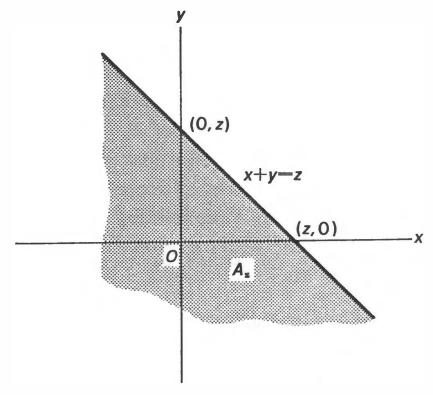
\includegraphics[width=\textwidth]{Imagens/soma.png}
    \caption{Imagem obtida de \cite{Hoel}.}
%    \label{fig:my_label}
\end{figure}
Em particular, se $X$ e $Y$ são duas v.a.'s independentes e não negativas, então
\begin{align*}
    f_{X+Y}(z) = \begin{cases}
    \int_0^z f_X(x)f_Y(z-x) dx, z > 0 \\
    0, \text{ c.c.}
    \end{cases}.
\end{align*}
Nesse caso, $f_{X+Y}$ é a \textbf{convolução} de $f_X$ e $f_Y$, denotada por $f_X*f_Y$.

\begin{example}
Sejam $X,Y$ v.a.'s i.i.d. com distribuição comum Exp($\lambda$). Note que $Z = X+Y$ é v.a. não negativa, de modo que $f_Z(z) = 0$ se $z\leq 0$. Para $z>0$, temos
\begin{align*}
    f_Z(z) = \int_0^z f_X(x)f_Y(z-x)dx = \int_0^z \lambda e^{-\lambda x}\lambda e^{-\lambda(z-x)} dx = \lambda^2 e^{-\lambda z}\int_0^z dx = \lambda^2 ze^{-\lambda z}.
\end{align*}
Logo,
\begin{align*}
    f_Z(z) = \begin{cases}
    \lambda^2z e^{-\lambda z}, z > 0 \\
    0, \text{ c.c.}
    \end{cases},
\end{align*}
ou seja, $Z\sim\Gamma(2,\lambda)$.
\end{example}

Esse exemplo tem uma generalização importante, enunciada como segue.

\begin{theorem}
Sejam $X$ e $Y$ v.a.'s independentes tais que $X\sim\Gamma(\alpha_1, \lambda)$ e $Y\sim\Gamma(\alpha_2, \lambda)$. Então $X+Y\sim\Gamma(\alpha_1+\alpha_2, \lambda)$.
\end{theorem}
\begin{proof}
Como $X$ e $Y$ são v.a.'s não negativas, segue que $f_{X+Y}(z) = 0, z\leq 0$. Para $z>0$, temos
\begin{align*}
    f_{X+Y}(z) &= \frac{ \lambda^{\alpha_1 + \alpha_2 e^{-\lambda z}} }{\Gamma(\alpha_1)\Gamma(\alpha_2)}\int_0^z x^{\alpha_1 - 1}(z-x)^{\alpha_2 - 1} dx \\
    &= \frac{\lambda^{\alpha_1+\alpha_2} z^{\alpha_1 + \alpha_2 - 1}e^{-\lambda z}}{\Gamma(\alpha_1)\Gamma(\alpha_2)}\int_0^1 u^{\alpha_1 - 1}(1-u)^{\alpha_2 - 1} du \\
    &= \frac{\lambda^{\alpha_1+\alpha_2} z^{\alpha_1 + \alpha_2 - 1}e^{-\lambda z}}{\Gamma(\alpha_1)\Gamma(\alpha_2)}\frac{ \Gamma(\alpha_1)\Gamma(\alpha_2) }{ \Gamma(\alpha_1 + \alpha_2) } \\
    &= \frac{\lambda^{\alpha_1+\alpha_2} z^{\alpha_1 + \alpha_2 - 1}e^{-\lambda z}}{\Gamma(\alpha_1+\alpha_2)},
\end{align*}
em que usamos que
\begin{align*}
    \int_0^1 u^{\alpha_1 - 1}(1-u)^{\alpha_2 - 1} du = \frac{ \Gamma(\alpha_1)\Gamma(\alpha_2) }{ \Gamma(\alpha_1+\alpha_2) }.
\end{align*}
Logo, $X+Y\sim\Gamma(\alpha_1+\alpha_2, \lambda)$.
\end{proof}

\begin{example}[Beta, $X\sim\text{Beta}(\alpha_1, \alpha_2)$]
A integral que usamos no argumento acima nos permite definir uma nova família de densidades, a dois parâmetros, chamadas \textbf{densidades betas}. Dizemos que $X$ tem densidade beta de parâmetros $\alpha_1$ e $\alpha_2$ (positivos) se sua densidade é dada por
\begin{align*}
    f_X(x) = \begin{cases}
    \frac{ \Gamma(\alpha_1+\alpha_2)x^{\alpha_1 - 1}(1-x)^{\alpha_2 - 1} }{ \Gamma(\alpha_1)\Gamma(\alpha_2) }, 0 < x < 1 \\
    0, \text{ c.c.}
    \end{cases}
\end{align*}
A nomenclatura ``beta'' vem do fato de que a função
\begin{align*}
    B(\alpha_1, \alpha_2) = \frac{ \Gamma(\alpha_1)\Gamma(\alpha_2) }{\Gamma(\alpha_1+\alpha_2)}, 0 < \alpha_1, \alpha_2 < \infty
\end{align*}
é chamada \textbf{função beta}.
\end{example}

\begin{example}
Sejam $X,Y$ i.i.d. com distribuição uniforme em $(0,1)$ e $Z=X+Y$. Note que $P((X,Y)\in (0,2)) = 1$, de modo que $f_{X+Y}(z) = 0$ se $z<0$ ou $z>2$. Se $0\leq z\leq 1$, então
\begin{align*}
    f_{X+Y}(z) = \int_0^z f_X(x)f_Y(z-x) dx = \int_0^z dx = z.
\end{align*}
Se $1 < z \leq 2$, então
\begin{align*}
    f_{X+Y}(z) = \int_0^z f_X(x)f_Y(z-x) dx = \int_{z-1}^{1} dx = 2 - z.
\end{align*}
Logo,
\begin{align*}
    f_{X+Y}(z) = \begin{cases}
    z, 0\leq z \leq 1 \\
    2-z, 1 < z \leq 2 \\
    0, \text{ c.c.}
    \end{cases}.
\end{align*}
\end{example}

Antes de passarmos à distribuição de quocientes, enunciamos um teorema importante acerca da soma de distribuições normais.

\begin{theorem}
Sejam $X$ e $Y$ v.a.'s independentes com $X\sim N(\mu_1, \sigma_1^2)$ e $Y\sim N(\mu_2, \sigma_2^2)$. Então $X+Y\sim N(\mu_1+\mu_2, \sigma_1^2 + \sigma_2^2)$.
\end{theorem}

\begin{proof}
Assumamos $\mu_1 = \mu_2 = 0$. Então
\begin{align*}
    f_{X+Y}(z) &= \frac{1}{2\pi\sigma_1\sigma_2}\int_{\mathbb{R}} \exp[ -\frac{1}{2}\left( \frac{x^2}{\sigma_1^2} + \frac{(z-x)^2}{\sigma_2^2} \right) ] dx \\
    &= \frac{1}{2\pi\sqrt{\sigma_1^2 + \sigma_2^2}}\int_{\mathbb{R}} \exp[ -\frac{1}{2}\left( u^2 - \frac{2uz\sigma_1}{\sigma_2\sqrt{\sigma_1^2 + \sigma_2^2}} + \frac{z^2}{\sigma_2^2} \right) ] du \\
    &= \frac{ e^{-z^2/2(\sigma_1^2+\sigma_2^2)} }{ \sqrt{2\pi}\sqrt{\sigma_1^2 + \sigma_2^2} }\int_{\mathbb{R}} \frac{e^{-v^2/2}}{\sqrt{2\pi}} dv \\
    &= \frac{ e^{-z^2/2(\sigma_1^2+\sigma_2^2)} }{ \sqrt{2\pi}\sqrt{\sigma_1^2 + \sigma_2^2} },
\end{align*}
em que fizemos a troca de variável
\begin{align*}
    u = \frac{\sqrt{\sigma_1^2 + \sigma_2^2}}{\sigma_1\sigma_2} x,
\end{align*}
completamos quadrados
\begin{align*}
    u^2 - \frac{2uz\sigma_1}{\sigma_2\sqrt{\sigma_1^2 + \sigma_2^2}} + \frac{z^2}{\sigma_2^2} = \left( u - \frac{z\sigma_1}{\sigma_2\sqrt{\sigma_1^2 + \sigma_2^2}} \right)^2 + \frac{z^2}{\sigma_1^2 + \sigma_2^2}
\end{align*}
e fizemos a segunda mudança de variável
\begin{align*}
    v = u - \frac{z\sigma_1}{\sigma_2\sqrt{\sigma_1^2 + \sigma_2^2}}.
\end{align*}
Notamos, então, que $X+Y\sim N(0, \sigma_1^2 + \sigma_2^2)$. Daí, de modo geral, $X-\mu_1$ e $Y-\mu_2$ também são independentes com densidades normais de parâmetros $0$ e $\sigma_1^2$ e $0$ e $\sigma_2^2$, respectivamente. Daí, $X+Y - (\mu_1 + \mu_2)$ tem densidade normal de parâmetros $\mu_1 + \mu_2$ e $\sigma_1^2 + \sigma_2^2$, como desejado.
\end{proof}

\paragraph{Distribuição do quociente.} Sejam $X$ e $Y$ v.a.'s com densidade conjunta $f$ e distribuição conjunta $F$. Estamos agora interessados em encontrar a distribuição de $Z=X/Y$. Note que dado $z\in\mathbb{R}$ fixo, temos
\begin{align*}
    \{Z\leq z\} = \{ (X,Y)\in A_z \},
\end{align*}
com
\begin{align*}
    A_z = \{ (x,y)\in\mathbb{R}^2 : y/x \leq z \} = \{ (x,y)\in\mathbb{R}^2 : x < 0, y\geq xz \} \cup \{ (x,y)\in\mathbb{R}^2 : x > 0, y\leq xz \}.
\end{align*}
\begin{figure}[H]
    \centering
    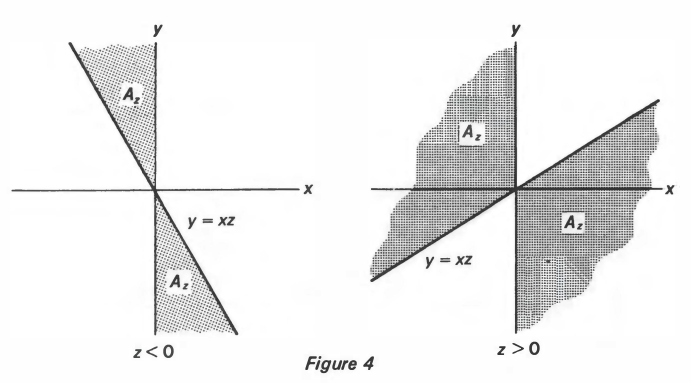
\includegraphics[width=\textwidth]{Imagens/quociente.png}
    \caption{Imagem obtida de \cite{Hoel}.}
%    \label{fig:my_label}
\end{figure}

Daí, segue que
\begin{align*}
    F_Z(z) = P(Z\leq z) = P((X,Y)\in A_z) &= \iint_{A_z} f(x,y) dxdy \\
    &= \int_{-\infty}^{0}\int_{xz}^{\infty} f(x,y) dydx + \int_{0}^{\infty}\int_{-\infty}^{xz} f(x,y) dydx \\
    &= \int_{-\infty}^{0}\int_{z}^{\infty} xf(x,xu) dudx + \int_{0}^{\infty}\int_{-\infty}^{z} xf(x,xu) dudx \\
    &= \int_{-\infty}^{0}\int_{-\infty}^{z} (-x)f(x,xu) dudx + \int_{0}^{\infty}\int_{-\infty}^{z} xf(x,xu) dudx \\
    &= \int_{\mathbb{R}}\int_{-\infty}^{z} |x|f(x,xu) dudx,
\end{align*}
donde segue que
\begin{align*}
    F_{Y/X}(z) = \int_{-\infty}^z \underbrace{\int_{\mathbb{R}} |x|f(x,xu) dx}_{f_{Y/X}(u)}du \implies f_{Y/X}(z) = \int_{\mathbb{R}} |x|f_{X,Y}(x,xz) dx, \forall z\in\mathbb{R}.
\end{align*}
Em  particular, se $X$ e $Y$ são independentes e não negativas, então
\begin{align*}
    f_{Y/X}(z) = \begin{cases}
    \int_{0}^{\infty} xf_X(x)f_Y(xz) dx, z > 0 \\
    0, z\leq 0
    \end{cases}.
\end{align*}

\begin{example}
Sejam $X$ e $Y$ v.a.'s independentes tais que $X\sim\Gamma(\alpha_1, \lambda)$ e $Y\sim\Gamma(\alpha_2, \lambda)$. Note que $X$ e $Y$ são não negativas, de modo que se $z\leq 0$ temos $f_{Y/X}(z) = 0$. Se $z>0$, então
\begin{align*}
    f_{Y/X}(z) = \int_{0}^{\infty} xf_X(x)f_Y(zx) dx &= \int_{0}^{\infty} x\frac{ \lambda^{\alpha_1}x^{\alpha_1 - 1}e^{-\lambda x} }{\Gamma(\alpha_1)}\frac{ \lambda^{\alpha_2}(xz)^{\alpha_2 - 1}e^{-\lambda xz} }{\Gamma(\alpha_2)} dx \\
    &= \frac{ \lambda^{\alpha_1+\alpha_2}z^{\alpha_2 - 1} }{\Gamma(\alpha_1)\Gamma(\alpha_2)} \int_{0}^{\infty} x^{\alpha_1 + \alpha_2 - 1}e^{-x\lambda (z+1)} dx \\
    &= \frac{ \Gamma(\alpha_1 + \alpha_2) }{ \Gamma(\alpha_1)\Gamma(\alpha_2) }\frac{z^{\alpha_2 - 1}}{(z+1)^{\alpha_1 + \alpha_2}},
\end{align*}
em que usamos que
\begin{align*}
    \int_{0}^{\infty} x^{\alpha_1 + \alpha_2 - 1}e^{-x\lambda (z+1)} dx = \frac{ \Gamma(\alpha_1+\alpha_2) }{[\lambda(z+1)]^{\alpha_1+\alpha_2}}.
\end{align*}
\end{example}

\begin{example}
Sejam $X,Y$ v.a.'s i.i.d. com distribuição $N(0, \sigma^2)$. Da Lista de Exercícios 7, sabemos que $X^2, Y^2\sim\Gamma(1/2, 1/2\sigma^2)$. Daí, do exemplo anterior, temos $f_{Y^2/X^2}(z) = 0$ se $z\leq 0$ e, para $z>0$, temos
\begin{align*}
    f_{Y^2/X^2}(z) = \frac{ \Gamma(1) }{ \Gamma(1/2)\Gamma(1/2) }\frac{z^{-1/2}}{z+1} = \frac{1}{\pi(z+1)\sqrt{z}}.
\end{align*}
Note também que dado $z\in\mathbb{R}$ qualquer, temos
\begin{align*}
    f_{Y/X}(z) &= 2\int_{0}^{\infty} xf_X(x)f_Y(xz) dx \\
    &= 2\frac{1}{2\pi\sigma^2}\int_{0}^{\infty} x\exp[ \frac{-x^2(1+z^2)}{2\sigma^2} ] dx \\
    &= \frac{1}{\pi\sigma^2}\frac{\sigma^2}{1+z^2}\int_{0}^{\infty} e^{-u} du \\
    &= \frac{1}{\pi(1+z^2)},
\end{align*}
ou seja, $Y/X\sim\text{Cauchy}(0,1)$. É possível mostrar também que $Y/|X|\sim\text{Cauchy}(0,1)$.
\end{example}

\begin{remark}
Podemos também falar de densidades condicionais e da Regra da Bayes no caso de v.a.'s contínuas; entretanto, optamos por não fazê-lo e focar nas distribuições clássicas de v.a.'s contínuas. Ao leitor interessado, consulte \cite{Hoel} pp. 153-157.
\end{remark}

Podemos ainda generalizar os exemplos da soma de v.a.'s gama e normal com os seguintes teoremas.

\begin{theorem}
Sejam $X_1, \dots, X_n$ v.a.'s independentes. Sejam $Y$ uma v.a. definida em termos de $X_1, \dots, X_m$ e $Z$ uma v.a. definida em termos de $X_{m+1}, \dots, X_n$, com $1\leq m < n$. Então $Y$ e $Z$ são independentes.
\end{theorem}

A prova deste teorema envolve argumentos de Teoria da Medida e, portanto, não será apresentada; entretanto, por indução e usando este teorema pode-se demonstrar os dois teoremas a seguir.

\begin{theorem}
Sejam $X_1, \dots, X_n$ v.a.'s independentes tais que $X_m\sim\Gamma(\alpha_m, \lambda)$, com $m=1,\dots,n$. Então $X_1 + \cdots + X_n\sim\Gamma(\alpha_1 + \cdots + \alpha_n, \lambda)$.
\end{theorem}

\begin{corollary}
Se $X_1, \dots, X_n$ são v.a.'s independentes com distribuição exponencial de parâmetro $\lambda$, então $X_1 + \cdots + X_n\sim\Gamma(n,\lambda)$.
\end{corollary}

\begin{theorem}
Sejam $X_1, \dots, X_n$ v.a.'s independentes tais que $X_m\sim N(\mu_m, \sigma_m^2)$, com $m=1,\dots,n$. Então $X_1 + \cdots + X_n\sim N(\mu_1 + \cdots + \mu_n, \sigma_1^2 + \cdots + \sigma_n^2)$.
\end{theorem}

\paragraph{Distribuição de vetores aleatórios bidimensionais.} Sejam $X$ e $Y$ v.a.'s contínuas com densidade conjunta $f_{X,Y}$. Considere $g_1:\mathbb{R}^2\to\mathbb{R}$ e $g_2:\mathbb{R}^2\to\mathbb{R}$ e tome
\begin{align*}
    \begin{cases}
    U = g_1(X,Y) \\
    V = g_2(X,Y)
    \end{cases}.
\end{align*}
Queremos determinar a distribuição conjunta de $U$ e $V$. Por definição,
\begin{align*}
    F_{U,V}(u,v) = P(U\leq u, V\leq v) = \iint_{B_{u,v}} f_{X,Y}(x,y) dxdy,
\end{align*}
com $B_{u,v} = \{ (x,y)\in\mathbb{R}^2 : g_1(x,y)\leq u, g_2(x,y)\leq v \}$. Em geral,
\begin{align*}
    f_{U,V}(u,v) = \frac{\partial^2}{\partial u\partial v} F_{U,V}(u,v).
\end{align*}
Em particular, podemos considerar
\begin{align*}
    \begin{cases}
    u = g_1(x,y) \\
    v = g_2(x,y)
    \end{cases}.
\end{align*}
Supondo que $g_1$ e $g_2$ têm derivadas parciais contínuas em todos os pontos e que
\begin{align*}
    J(x,y) = \begin{vmatrix}
    \frac{\partial}{\partial x} g_1 & \frac{\partial}{\partial y} g_1 \\
    \frac{\partial}{\partial x} g_2 & \frac{\partial}{\partial y} g_2
    \end{vmatrix}\neq 0,
\end{align*}
então pelo teorema da função inversa podemos resolver (localmente) o sistema acima, ou seja, existem $h_1, h_2:\mathbb{R}^2\to\mathbb{R}$ tais que
\begin{align*}
    \begin{cases}
    x = h_1(u,v) \\
    y = h_2(u,v)
    \end{cases}.
\end{align*}
Logo, $U$ e $V$ são v.a.'s contínuas com densidade conjunta
\begin{align*}
    f_{U,V}(u,v) = \frac{1}{|J(x,y)|}f_{X,Y}(x,y),
\end{align*}
com $x,y$ dados como acima. Ademais,
\begin{align*}
    F_{U,V}(u,v) = \int_{-\infty}^u\int_{-\infty}^v f_{U,V}(z,w) dwdz.
\end{align*}

\begin{example}
Sejam $X,Y$ i.i.d. com distribuição exponencial de parâmetro $\lambda$ e 
\begin{align*}
    \begin{cases}
    U = X+Y \\
    V = X-Y
    \end{cases}.
\end{align*}
Note que $P(U>0) = 1$ e $P(V\in\mathbb{R}) = 1$. Daí,
\begin{align*}
    \begin{cases}
    u = x+y \\
    v = x-y
    \end{cases} \implies 
    \begin{cases}
    x = \frac{u+v}{2} \\
    y = \frac{u-v}{2}
    \end{cases}, u > 0 \text{ e } -u < v < u.
\end{align*}
Ademais, $\displaystyle{ J = \begin{vmatrix} 1 & 1 \\
1 & -1 \end{vmatrix} = -2}$. Logo, para $u>0$ e $-u < v < u$, temos
\begin{align*}
    f_{U,V}(u,v) = \frac{1}{|J|}f_{X,Y}\left(\frac{u+v}{2}, \frac{u-v}{2} \right) = \frac{1}{|J|}f_X\left(\frac{u+v}{2}\right)f_Y\left(\frac{u-v}{2}\right) = \frac{\lambda^2}{2}e^{-\lambda u},
\end{align*}
ou seja,
\begin{align*}
    f_{U,V}(u,v) = \begin{cases}
    \frac{\lambda^2}{2}e^{-\lambda u}, u > 0 \text{ e } -u < v < u \\
    0, \text{ c.c.}
    \end{cases}.
\end{align*}
Daí, dado $u>0$, temos
\begin{align*}
    f_U(u) = \int_{\mathbb{R}} f_{U,V}(u,v) dv = \int_{-u}^{u} \frac{\lambda^2}{2}e^{-\lambda u} dv = \lambda^2 ue^{-\lambda u},
\end{align*}
ou seja,
\begin{align*}
    f_U(u) = \begin{cases}
    \lambda^2 ue^{-\lambda u}, u > 0 \\
    0, \text{ c.c.}
    \end{cases} \therefore U\sim\Gamma(2, \lambda).
\end{align*}
Ademais, dado $v\in\mathbb{R}$,
\begin{align*}
    f_V(v) = \int_{\mathbb{R}} f_{U,V}(u,v) du = \begin{cases}
    \int_{v}^{\infty} \frac{\lambda^2}{2} e^{-\lambda u} du = \frac{\lambda}{2}e^{-\lambda v}, v > 0 \\
    \int_{-v}^{\infty} \frac{\lambda^2}{2} e^{-\lambda u} du = \frac{\lambda}{2}e^{-\lambda (-v)}, v < 0
    \end{cases},
\end{align*}
ou seja,
\begin{align*}
    f_V(v) = \frac{\lambda}{2}e^{-\lambda |v|}, \forall v\in\mathbb{R}.
\end{align*}
\end{example}

\begin{example}
Sejam $X$ e $Y$ v.a.'s i.i.d. exponenciais de parâmetro $\lambda$ e $Z = X+3Y$. Considere $U = X$. Daí,
\begin{align*}
    \begin{cases}
    u = x \\
    z = x + 3y
    \end{cases}\implies
    \begin{cases}
    x = u \\
    y = \frac{z-u}{3}
    \end{cases}, z > 0 \text{ e } 0 < u < z.
\end{align*}
Ademais, $J = 3$. Logo, dados $z>0$ e $0<u<z$, temos
\begin{align*}
    f_{U,Z}(u,z) = \frac{\lambda^2}{3} e^{-2\lambda/3}e^{-\lambda z/3}
\end{align*}
e, se $z\leq 0$ ou $u \leq 0$ ou $u\geq z$, $f_{U,Z}(u,z) = 0$. Daí, dado $z>0$, temos
\begin{align*}
    f_Z(z) = \int_0^z \frac{\lambda^2}{3} e^{-2\lambda/3}e^{-\lambda z/3} du = \frac{\lambda}{2}(e^{-\lambda z/3} - e^{-\lambda z})
\end{align*}
e $f_Z(z) = 0$ se $z\leq 0$.
\end{example}

\begin{remark}
Podemos ainda generalizar esse método do jacobiano para $n$ variáveis, de maneira natural:
\begin{align*}
    f_{Y_1, \dots, Y_n}(y_1, \dots, y_n) = \frac{1}{|J(x_1, \dots, x_n)|}f(x_1, \dots, x_n),
\end{align*}
com os $x_i$'s definidos implicitamente pelos $y_j$'s por
\begin{align*}
    y_i = g_i(x_1, \dots, x_n), i = 1,\dots,n,
\end{align*}
e o jacobiano é a matriz $n\times n$ generalizada naturalmente do jacobiano $2\times 2$.
\end{remark}

\section{Esperança de variáveis aleatórias contínuas}
\begin{definition}
Seja $X$ v.a. contínua com densidade $f_X$. Definimos a \textbf{esperança} de $X$ por
\begin{align*}
    EX = \int_{\mathbb{R}} xf_X(x) dx,
\end{align*}
desde que a integral exista, isto é, seja bem definida.
\end{definition}
\begin{remark}
Dizemos que $EX$ é bem definida quanto podemos escrever
\begin{align*}
    EX = \int_{\mathbb{R}} xf_X(x) dx = \int_{0}^{\infty} xf_X(x) dx - \int_{-\infty}^0 -xf_X(x) dx
\end{align*}
e quando não ocorre a indefinição $\infty - \infty$. Note que $EX < \infty$ sempre que $\displaystyle{ \int_{0}^{\infty} xf_X(x) dx }$ e $\displaystyle{ \int_{-\infty}^{0} xf_X(x) dx }$ forem finitas. Ademais, como veremos mais à frente, $EX < \infty \iff E|X| < \infty$.
\end{remark}

\begin{example}
Seja $X\sim U(a,b)$. Temos
\begin{align*}
    \int_{\mathbb{R}} xf_X(x) dx = \int_a^b \frac{x}{b-a} dx = \frac{a+b}{2}\in\mathbb{R} \therefore EX = \frac{a+b}{2}.
\end{align*}
\end{example}

\begin{example}
Seja $X\sim\text{Exp}(\lambda)$. Temos
\begin{align*}
    \int_{\mathbb{R}} xf_X(x) dx &= \int_{0}^{\infty} x\lambda e^{-\lambda x} dx \\
    &= \lambda\left[ -\frac{xe^{-\lambda x}}{\lambda}\Big|_0^{\infty} + \frac{1}{\lambda}\int_{0}^{\infty} e^{-\lambda x}dx \right] \\
    &= \frac{1}{\lambda}\in\mathbb{R}\therefore EX = \frac{1}{\lambda}.
\end{align*}
\end{example}

\begin{example}
Seja $X\sim\Gamma(\alpha, \lambda)$. Temos
\begin{align*}
    \int_{\mathbb{R}} xf_X(x) dx &= \int_{0}^{\alpha} x\frac{\lambda^{\alpha}}{\Gamma(\alpha)}x^{\alpha - 1}e^{-\lambda x} dx \\
    &= \frac{\lambda^{\alpha}}{\Gamma(\alpha)}\int_{0}^{\infty} x^{\alpha}e^{-\lambda x} dx \\
    &= \frac{\lambda^{\alpha}}{\Gamma(\alpha)}\frac{\Gamma(\alpha + 1)}{\lambda^{\alpha + 1}} \\
    &= \frac{\alpha}{\lambda} \in\mathbb{R} \therefore EX = \frac{\alpha}{\lambda}.
\end{align*}
\end{example}

\begin{example}
Seja $X\sim\text{Cauchy}(0,1)$. Temos
\begin{align*}
    \int_{\mathbb{R}} xf_X(x) dx = \frac{1}{\pi}\int_{0}^{\infty} \frac{x}{1+x^2} dx + \frac{1}{\pi}\int_{-\infty}^{0} \frac{x}{1+x^2} dx = \frac{1}{2\pi}\left[ \underbrace{\int_{0}^{\infty} \frac{1}{u}du - \int_{0}^{\infty} \frac{1}{u}du}_{\infty - \infty} \right],
\end{align*}
logo não existe $EX$.
\end{example}

\begin{remark}
Com a noção de densidade condicional, é possível também definir uma \textbf{esperança condicional}. Como não tratamos de densidades condicionais, também não trataremos de esperanças condicionais.
\end{remark}

\subsection{Esperança de função de variável aleatória contínua}
Sejam $X$ v.a contínua com densidade $f_X$ e $Y = \varphi(X)$, sendo $\varphi:\mathbb{R}\to\mathbb{R}$ função. Por definição, $Y$ tem esperança finita se, e só se,
\begin{align*}
    \int_{\mathbb{R}} |y|f_Y(y) dy < \infty 
\end{align*}
e, nesse caso,
\begin{align*}
    EY = \int_{\mathbb{R}} yf_Y(y) dy < \infty.
\end{align*}
No caso de $\varphi$ ser discreta, temos $Y$ v.a. discreta e podemos aplicar os resultados vistos anteriormente sobre esperanças de v.a.'s discretas para calcular $EY$. No caso de $\varphi$ ser tal que $Y$ é v.a. contínua, temos que $Y$ tem esperança finita se, e só se,
\begin{align*}
    \int_{\mathbb{R}} |\varphi(x)|f_X(x) dx < \infty
\end{align*}
e, nesse caso,
\begin{align*}
    EY = \int_{\mathbb{R}} \varphi(x)f_X(x) dx < \infty.
\end{align*}
De maneira geral, dadas $X_1, \dots, X_n$ v.a.'s contínuas com densidade conjunta $f_{X_1, \dots, X_n}$ e $\varphi:\mathbb{R}^n\to\mathbb{R}$ função real de modo que $Y = \varphi(X_1, \dots, X_n)$ tem densidade, então
\begin{align*}
    EY < \infty \iff \int_{\mathbb{R}}\cdots\int_{\mathbb{R}} |\varphi(x_1, \dots, x_n)|f_{X_1, \dots, X_n}(x_1, \dots, x_n) dx_1\cdots dx_n < \infty
\end{align*}
e, nesse caso,
\begin{align*}
    EY = \int_{\mathbb{R}}\cdots\int_{\mathbb{R}} \varphi(x_1, \dots, x_n)f_{X_1, \dots, X_n}(x_1, \dots, x_n) dx_1\cdots dx_n < \infty.
\end{align*}

\begin{example}
Sejam $X\sim U(0,1)$ e $Y=X^2$. Temos
\begin{align*}
    EY = E[X^2] = \int_{\mathbb{R}}x^2f_X(x) dx = \int_0^1 x^2 dx = 1/3.
\end{align*}
\end{example}

\begin{example}
Sejam $X$ e $Y$ v.a.'s contínuas com densidade conjunta $f_{X,Y}$ e suponha que $EX,EY<\infty$. Seja $Z=X+Y$. Temos
\begin{align*}
    \int_{\mathbb{R}}\int_{\mathbb{R}} xf_{X,Y}(x,y) dxdy = \int_{\mathbb{R}} x\int_{\mathbb{R}} f_{X,Y}(x,y) dy dx = \int_{\mathbb{R}} xf_X(x) dx = EX < \infty.
\end{align*}
Analogamente,
\begin{align*}
    \int_{\mathbb{R}}\int_{\mathbb{R}} yf_{X,Y}(x,y) dxdy = EY < \infty.
\end{align*}
Logo,
\begin{align*}
    EZ = E[X+Y] = \int_{\mathbb{R}}\int_{\mathbb{R}} (x+y)f_{X,Y}(x,y) dxdy = \int_{\mathbb{R}}\int_{\mathbb{R}} xf_{X,Y}(x,y) dxdy + \int_{\mathbb{R}}\int_{\mathbb{R}} yf_{X,Y}(x,y) dxdy = EX + EY.
\end{align*}
\end{example}

\begin{proposition}[Propriedades da esperança]
Sejam $X$ e $Y$ v.a.'s contínuas com $E|X|, E|Y| < \infty$. Temos
\begin{enumerate}[(i)]
    \item $P(X=c) = 1 \implies EX = c, c\in\mathbb{R}$
    \item $E[cX] = cEX, \forall c\in\mathbb{R}$
    \item $E[X+Y] = EX + EY$
    \item $|EX| \leq E|X|$
    \item se $X,Y$ são independentes, então $E[XY] = EXEY$
    \item se $P(X\geq Y) = 1$, então $EX\geq EY$; em particular, $P(X=Y) = 1\iff EX = EY$
    \item se $P(|X|\leq M) = 1$ para algum $M$ real positivo, então $|EX|\leq M$.
\end{enumerate}
\end{proposition}

\begin{proof}
As demonstrações são análogas ao caso discreto.
\end{proof}

\subsection{Momentos de uma variável aleatória contínua}
Seja $X$ v.a. contínua com densidade $f_X$.
\begin{definition}
\begin{enumerate}[(i)]
    \item Dado $k\in\mathbb{N}$, $E[X^k]$ é o \textbf{momento de ordem} $k$ de $X$ ou $k$\textbf{-ésimo momento} de $X$.
    \item Dado $k\in\mathbb{N}$ e sendo $EX<\infty$, $E[(X-EX)^k]$ é o \textbf{momento central de ordem} $k$ de $X$ ou $k$\textbf{-ésimo momento central} de $X$. Em particular, $\Var(X) = E[(X-EX)^2]$ é a \textbf{variância} de $X$ e $\sigma = \sqrt{\Var(X)}$ é o \textbf{desvio-padrão} de $X$.
    \item Dado $k\in\mathbb{N}$, $E|X|^k$ é o \textbf{momento absoluto de ordem} $k$ de $X$ ou $k$\textbf{-ésimo momento absoluto} de $X$.
\end{enumerate}
\end{definition}

\begin{remark}
Se $EX = \mu\in\mathbb{R}$, então
\begin{align*}
    \Var(X) = \sigma^2 = \int_{\mathbb{R}} (x-\mu)^2 f_X(x) dx.
\end{align*}
Daí, mostra-se que
\begin{itemize}
    \item $\Var(X) = E[X^2] - EX^2 = E[X^2] - \mu^2$
    \item $\sigma^2 = 0 \iff P(X=\mu) = 1$, logo se $X$ é v.a. contínua então $\Var(X) > 0$
    \item $E[|X|^k]<\infty \implies E[|X|^j]<\infty, \forall j\leq k$.
\end{itemize}
\end{remark}

\begin{example}
Seja $X\sim\Gamma(\alpha, \lambda)$. Vimos que $EX = \alpha/\lambda$. Ademais, dado $k\in\mathbb{N}$, temos
\begin{align*}
    E[X^k] = \int_{0}^{\infty} x^k\frac{\lambda^{\alpha}}{\Gamma(\alpha)}x^{\alpha - 1}e^{-\lambda x} dx = \frac{\lambda^{\alpha}}{\Gamma(\alpha)}\int_{0}^{\infty} x^{k+\alpha - 1}e^{-\lambda x} dx = \frac{\Gamma(a+k)}{\Gamma(\alpha)}\frac{1}{\lambda^k} = \frac{\alpha(\alpha+1)\cdots(\alpha+k-1)}{\lambda^k}.
\end{align*}
Em particular, segue daí que $\Var(X) = \alpha/\lambda^2$. Além disso, se $X\sim\chi^2(n)$, isto é, $X\sim\Gamma(n/2, 1/2)$, então $EX = n$ e $\Var(X) = 2n$. Por fim, se $\alpha = 1$, então $X\sim\text{Exp}(\lambda)$ e temos $E[X^k] = k!/\lambda^k$ e $\Var(X) = 1/\lambda^2$.
\end{example}

\begin{example}
Seja $X$ v.a. contínua com densidade simétrica $f_X$. Suponha que $E[X^k] < \infty$. Então $\displaystyle{ \int_{0}^{\infty} x^k f_X(x) dx < \infty}$ e $\displaystyle{ \int_{-\infty}^{0} x^k f_X(x) dx < \infty}$. Logo,
\begin{align*}
    \int_{-\infty}^{0} x^k f_X(x) dx = \int_{0}^{\infty} (-u)^k f_X(-u) du = \int_{0}^{\infty} (-u)^k f_X(u) du,
\end{align*}
ou seja,
\begin{align*}
    E[X^k] = \int_{0}^{\infty} x^k f_X(x) dx + \int_{0}^{\infty} (-x)^k f_X(x) dx .
\end{align*}
Portanto,
\begin{align*}
    E[X^k] = \begin{cases}
    2\int_{0}^{\infty} xf_X(x) dx, k \text{ par} \\
    0, k \text{ ímpar}
    \end{cases}.
\end{align*}
\end{example}

\begin{example}
\begin{enumerate}[a)]
    \item Seja $X\sim N(0, \sigma^2)$. Note que $f_X$ é simétrica, de modo que $E[X^k] = 0$ se $k$ ímpar; para $k$ par, como $X^2\sim\Gamma(1/2, 1/2\sigma^2)$, então
\begin{align*}
    E[X^k] = E[(X^2)^m] &= \frac{ \Gamma(m+1/2) }{\Gamma(1/2)}\frac{1}{(1/2\sigma^2)^m} \\
    &= \frac{ \Gamma\left(\frac{k+1}{2}\right) }{ \Gamma(1/2) }\frac{1}{(1/2\sigma^2)^{k/2}} \\
    &= \frac{1}{\sqrt{\pi}}\frac{\sqrt{\pi} k!}{2^k (k/2)!}\frac{1}{\frac{1}{2^{k/2}\sigma^k}} \\
    &= \frac{k!}{2^{k/2}(k/2)!}\sigma^k.
\end{align*}
    \item Seja $X\sim N(\mu, \sigma^2)$, de modo que $X-\mu\sim N(0, \sigma^2)$. Se $k$ é ímpar, então $E[(X-\mu)^k] = 0 \implies E[X-\mu] = 0 \implies EX = \mu$. Se $k$ é par, 
    \begin{align*}
        E[(X-\mu)^k] = \frac{k!\sigma^k}{2^{k/2}(k/2)!}.
    \end{align*}
    Daí, $\Var(X-\mu) = E[(X-\mu)^2] = \sigma^2$.
\end{enumerate}
\end{example}

\begin{definition}[Covariância e correlação]
Sejam $X$ e $Y$ v.a.'s tais que $EX, EY < \infty$. A \textbf{covariância} de $X$ e $Y$ é definida por
\begin{align*}
    \Cov(X,Y) := E[(X-EX)(Y-EY)] = E[XY] - EXEY.
\end{align*}
Se $X$ e $Y$ são v.a.'s contínuas com densidade conjunta $f_{X,Y}$, então
\begin{align*}
    \Cov(X,Y) = \iint_{\mathbb{R}^2} (x-EX)(y-EY)f_{X,Y}(x,y) dxdy.
\end{align*}
Se além de $EX, EY < \infty$ tivermos $0 < E[X^2], E[Y^2] < \infty$, definimos a \textbf{correlação} entre $X$ e $Y$ por
\begin{align*}
    \rho(X,Y) := \frac{\Cov(X,Y)}{\sqrt{\Var(X)}\sqrt{\Var(Y)}}.
\end{align*}
\end{definition}

\begin{remark}
As mesmas propriedades da covariância e da correlação para v.a.'s discretas valem para v.a.'s contínuas: 
\begin{enumerate}[(a)]
    \item se $X$ e $Y$ são v.a.'s contínuas independentes, então $\Cov(X,Y) = 0$ e, portanto, $\rho(X,Y) = 0$, mas a recíproca é falsa pelo mesmo raciocínio do caso discreto;
    \item se $X_1, \dots, X_n$ são v.a.'s contínuas independentes tais que $0 < E[X_i^2] < \infty, i = 1, \dots, n$, então
    \begin{align*}
        \Var(X_1 + \cdots + X_n) = \sum_{i=1}^n \Var(X_i) + 2\sum_{i=1}^{n-1}\sum_{j=i+1}^{n}\Cov(X_i, X_j).
    \end{align*}
    Se as v.a.'s são independentes, então
    \begin{align*}
        \Var(X_1 + \cdots + X_n) = \sum_{i=1}^n \Var(X_i)
    \end{align*}
    \item se $X$ e $Y$ são v.a.'s contínuas com segundo momento finito e positivo, então vale a desigualdade de Cauchy-Schwarz,
    \begin{align*}
        E[XY]^2 \leq E[X^2]E[Y^2]
    \end{align*}
    e, daí,
    \begin{align*}
        \Cov(X,Y)^2 \leq \Var(X)\Var(Y) \implies |\rho(X,Y)| \leq 1.
    \end{align*}
\end{enumerate}
\end{remark}

\begin{example}
Sejam $X$ e $Y$ v.a.'s com densidade conjunta
\begin{align*}
    f_{X,Y}(x,y) = \frac{\sqrt{3}}{4\pi}\exp[ -\frac{x^2 - xy + y^2}{2} ], \forall (x,y)\in\mathbb{R}^2.
\end{align*}
Vimos que $X,Y\sim N(0, 4/3)$, mas não eram independentes. Logo, $EX = 0 = EY$ e $\Var(X) = 4/3 = \Var(Y)$. Temos também
\begin{align*}
    E[XY] = \iint_{\mathbb{R}^2} xyf_{X,Y}(x,y) dxdy &= \sqrt{2\pi}\frac{\sqrt{3}}{4\pi}\int_{\mathbb{R}} xe^{-3x^2/8}\left( \frac{1}{\sqrt{2\pi}} y\exp[ -\frac{1}{2}\left( y - \frac{x}{2} \right)^2 ] dy\right) dx \\
    &= \frac{\sqrt{6}}{8\sqrt{\pi}} \int_{\mathbb{R}} x^2e^{-3x^2/8} dx \\
    &= \frac{\sqrt{6}}{8\sqrt{\pi}}\sqrt{2\pi}\sqrt{\frac{4}{3}}\int_{\mathbb{R}} \frac{1}{\sqrt{2\pi}\sqrt{4/3}} x^2 \exp[ -\frac{1}{2}\frac{x^2}{4/3} ] dx \\
    &= \frac{\sqrt{6}}{8\sqrt{\pi}}\sqrt{2\pi}\sqrt{\frac{4}{3}}\frac{4}{3} \\
    &= \frac{2}{3}.
\end{align*}
Logo, $\Cov(X,Y) = E[XY] - EXEY = 2/3$ e 
\begin{align*}
    \rho(X,Y) = \frac{2/3}{\sqrt{4/3}\sqrt{4/3}} = \frac{1}{2}.
\end{align*}
\end{example}

\end{document}